\chapter{Traffic Light Matching}\label{ch:matching}

\begin{Summary}[Bibliographical Notes]
This chapter is based on the following two papers in which the author was the principal investigator: 

\cite{matthes2022matching} \fullcite{matthes2022matching}

\cite{matthes2023geo} \fullcite{matthes2023geo}

This chapter integrates concepts and results from a Master thesis, where the author identified the topic and was also involved as the primary supervisor:

\cite{jeschor_2022} \fullcite{jeschor_2022}
\end{Summary}

\section{Introduction}

Accurately detecting upcoming traffic lights is crucial for many driving applications. It is a safety-critical functionality for (semi)autonomous driving systems and essential for bridging the gap between traffic light prediction and speed recommendation. So far, we have considered the traffic light prediction without its relationship to the traffic light's position along the user's trajectory. However, to provide a speed advisory, we must not only know about the predicted timing of the traffic light but also its position and whether it aligns with the predicted path. A georeferencing is required.

The concept of georeferencing intersections, initially abbreviated under Geometric Intersection Description (GID), was introduced relatively early in the USA in 2008 \cite{cicas-v}. To reference the position of traffic lights and the specific turns they serve, the turn lane shapes are represented as line geometries crossing the intersection. In this way, it is possible to distinguish between turn directions and find which traffic light will be relevant for the vehicle. Today, this information is represented in the internationally standardized MapData (MAP) format that was developed by the SAE\footnote{\url{https://www.sae.org/standards/content/j2735_202309/}} in coevolution with the Signal Phase and Timing (SPaT) message standard.

MAPs, like SPaTs, can reach the road user through various channels, encountering similar transmission issues as SPaTs (see \Cref{ch:prediction}). However, since MAPs are less frequently updated, collecting, transferring to a database, and redistributing the lane geometries is possible. This aspect makes it viable to maintain a centralized directory service in which each lane is mapped. In Hamburg, the Traffic Lights Data platform provides this centralized directory service, which takes information from the MAPs developed mainly by engineering bureaus for Hamburg's intersections.

A more significant challenge than acquiring intersection topologies is determining which lane on the intersection will be used by a road user approaching it. Typically, multiple individual paths can be chosen when crossing an intersection, and the concrete choice may depend on the user's route, mode of transportation, situation, or general preference. Due to the complexity of real-world traffic, a sudden lane change to align with the traffic perceived as the best option is possible, requiring the system to adapt quickly to the new lane or anticipate the direction the user wants to travel. 

While cars are usually restricted by a few available lanes, cyclists or pedestrians often have multiple ambiguous options to cross an intersection toward the same destination. Moreover, cyclists or pedestrians may approach a traffic light from several directions, leading to no clear ingress lane. This uncertainty leads to the issue that the user's position cannot simply be matched to the nearest ingress lane geometry. Therefore, the problem of matching the correct traffic lights is highly complex, and even more so for cyclist applications.

This chapter aims to address this problem and develop a practical solution for cyclist traffic light matching. First, we review related work and how they address the problem, identifying three core approaches: vision-based using cameras or similar sensors for traffic light identification, location-based using global navigation and satellite systems (GNSS) for lane positioning, and route-based using semantic information such as turns for lane selection. We find that route-based approaches are currently the most promising for bicycle applications. 

Based on this finding, two new route-based traffic light matching methods are proposed: algorithmic and Machine Learning (ML) methods. We also focus on approaches that did not yield the desired results and the reasons behind them. Finally, we evaluate the accuracy of the developed approach using multiple ground truths to make well-founded statements about the method's suitability. A critical summary of the state-of-the-art, developed methods and results is provided to indicate future work directions.

\section{Related Work}

How traffic light matching is implemented differs significantly between simulation and real-world studies. Simulation environments usually have an inbuilt capability to determine the upcoming traffic light for each vehicle agent. SUMO, the most popular simulation environment among GLOSA studies \cite{krajzewicz_preparing_2012, erdmann_combining_2013, eckhoff_potentials_2013, tal_vehicular-communications-based_2016, nguyen_efficient_2016, olaverri-monreal_implementation_2018, karoui_efficiency_2018, pariota_green_2019, kloeppel_performance_2019, lu_green_2020, halbach_cooperative_2021, bhattacharyya_assessing_2022, grumert_heads-up_2022, wagner_spatmap_2023}, offers a specialized API for traffic light matching as part of the TraCI\footnote{\url{https://sumo.dlr.de/docs/TraCI.html}} interface. This interface is utilized by Krajzewicz et al. (2011) \cite{krajzewicz_preparing_2012}, Klöppel et al. (2019) \cite{kloeppel_performance_2019}, Halbach et al. (2021) \cite{halbach_cooperative_2021}, Grumert and Pereira (2022) \cite{grumert_heads-up_2022}, Wagner et al. (2023) \cite{wagner_spatmap_2023}, and Schlamp et al. (2023) \cite{schlamp_2023_glosa}, allowing the authors to find upcoming traffic lights through the simulation environment which knows about the relation between the path network and each traffic light. Some studies also assume that only one traffic light is associated with each ingress direction at the intersection \cite{xia_indirect_2011, li_multi-vehicles_2014, plianos_predictive_2018}.

However, these methods only apply to the real world to a limited extent. While, in general, the easiest option here is preselecting the traffic lights in advance, this may be only possible in test track environments with a predefined vehicle route and only a few intersections \cite{chen_developing_2022} or corridors \cite{fickas_fast_2019}. Since an approach is desired in which users can travel freely throughout the city, other methods to find appropriate traffic lights must be identified. The following sections will discuss three possible solutions: vision-based, location-based, and route-based approaches.

\subsection{Vision-Based Approaches}

Vision-based approaches primarily originate from the field of autonomous driving. The concept involves utilizing sensors such as radar, cameras, LiDAR, and, in some cases, GNSS to perceive the surrounding environment and identify lanes \cite{lee_avm_2017} \cite{sadli_map-matching-based_2022}. Simultaneous Localization and Mapping (SLAM) is a method within this category that focuses on accurately mapping the environment and locating the vehicle within \cite{cheng_review_2022}. While SLAM captures the environment in real-time, there are also ground truths, known as HD-Maps \cite{kang_lane-level_2020}. Examples of such HD maps include TomTom HD Maps\footnote{\url{https://www.tomtom.com/products/hd-map/}}, NVIDIA DRIVE Map\footnote{\url{https://www.nvidia.com/de-de/self-driving-cars/hd-mapping/}}, or HERE HD Map\footnote{\url{https://www.here.com/platform/HD-live-map}}. These maps provide detailed semantic information, including lane positions and key objects such as traffic lights, and are primarily used for trajectory planning in autonomous vehicles. However, these approaches are largely impractical for smartphones due to availability, sensor, and computational constraints.

An approach practical for smartphones is presented by Koukoumidis et al. (2011–2012) \cite{koukoumidis_signalguru_2011, koukoumidis_leveraging_2012}. By mounting the smartphone on the car's windshield, the position and relevance of traffic lights for speed recommendations are detected only using the smartphone's camera and the user's movement direction. Additionally, the color of the traffic light is detected to obtain its state directly without needing an external data source. In a collaborative approach, information about traffic light phases is gathered as users pass by, and a prediction is estimated from the sparse crowdsourced data. The designed camera system achieves a per-camera-frame detection accuracy of 87.6\% to 92.2\%, depending on the deployment location and the number of frames recorded standing at a red light. This accuracy could certainly be improved with the object recognition methods available today. However, the main limitation lies elsewhere. Like other vision-based approaches from the field of autonomous driving, the main limitation of this approach is its reliance on a clear line of sight. A handlebar-mounted or stowed-away smartphone, such as in the case of a bike-GLOSA app, does not provide this line of sight. Consequently, vision-based approaches are generally attractive for autonomous driving or car applications but not for bikes.

\subsection{Location-Based Approaches}

Location-based approaches circumvent the issue of requiring a line-of-sight to the traffic light since they only depend on a GNSS location and intersection topologies. The first study identified to express this idea is a technical report by the US Research and Innovative Technology Administration in 2008 \cite{cicas-v}. This report describes a location-based traffic light matching system as part of a Cooperative Intersection Collision Avoidance System (CICAS-V). The described method is relatively simple: as a vehicle approaches the intersection topology, it determines which lane geometries are closest to its position and angle. The closest lane is determined to be relevant for the traffic light service.

Katsaros et al. (2011) \cite{katsaros_performance_2011} were the first to employ this method for a GLOSA system. In their study, the location of each traffic light is extracted from an obtained topology message and compared to the vehicle's position and heading. Notably, even though the study was conducted in a SUMO simulation environment, the authors did not rely on data from the simulation environment itself. Unfortunately, no further detail is given on the approach's procedure and accuracy.

Bernais et al. (2016) \cite{bernais_design_2016} describe a similar approach in a real-world GLOSA system for Braunschweig, Düsseldorf, and Kassel. Instead of matching an individual lane, their approach includes matching upcoming traffic lights based on their stop line. This workaround reduces the complexity of the matching problem significantly since the vehicle's heading can be roughly compared to each ingress direction at the upcoming intersection instead of comparing the position to each lane. On the other hand, the stop-line method introduces the need for a multi-lane presentation of the speed advisory since no decision on a specific traffic light is made. This approach is also used by Yunex's traffic light service "APHA" according to the technical documentation \cite{yunex_traffic_v2x-kommunikation_2023}. Other studies, such as by Khan et al. (2021) \cite{khan_eco-drive_2021}, or also the TrafficPilot app, presumably use a similar approach due to the designed user interface. However, it is unclear if this assumption is valid due to the lack of methodological details and reported results. Thus, it is not easy to reproduce or judge this approach.

Wilson et al. (2017) \cite{wilson_driver_2017}, developing BMW's EnLighten system, studied how a smartphone's inbuilt GNSS positioning could determine the upcoming traffic light. Again, not much is known about the concrete traffic light matching method. However, this study contributes to understanding which challenges a location-based approach may impose in real-world deployments. Wilson et al. (2017) \cite{wilson_driver_2017} were the first to report issues with the smartphone's GNSS. Any issues with the smartphone's GNSS are problematic since the location-based approach assumes that the GNSS is accurate enough and always available to determine the vehicle's position on a lane. However, in their study, the GLOSA system would regularly shut down due to losing GNSS connectivity. As the authors reported, this problem leads to user frustration and degraded usability, depending on the malfunctioning rate. A key conclusion is that a perfect GNSS availability cannot always be assumed. 

The GNSS accuracy was determined as another core issue by Stahlmann et al. (2018) \cite{stahlmann_exploring_2018} studying the real-world challenges associated with Audi's GLOSA system. Due to inaccurate geolocation, a similar problem was observed, namely that the system would not enable itself correctly on some occasions since the correct lane could not be identified. Methodologically, the author's approach is equal to the approach described in 2008. However, one variation was included. The car's turn indicator state was incorporated to resolve some ambiguities in the lane selection, especially with multiple parallel lanes. The information about this indicator was fetched from the car's local information network (CAN bus). Therefore, this workaround is strongly tied to a car environment.

A similar issue with the location-based approach was identified by Bhattacharyya et al. (2022) \cite{bhattacharyya_assessing_2022}, who also observed lane mismatching due to the limited GNSS accuracy. In contrast, the authors distinguished the matching inaccuracies in one more category: horizontal mismatching and vertical mismatching. While horizontal mismatching refers to the failing detection of the correct traffic light lane, vertical mismatching refers to the problem that intersection topologies may lack the needed height information to distinguish over- and underpasses. Due to this issue, there may be cases where lanes on overpasses or underpasses are not detected correctly.

Bhattacharyya et al. (2022) \cite{bhattacharyya_assessing_2022} propose addressing horizontal mismatching with improved GNSS accuracy. However, which specific methods could be utilized and are practical for a smartphone app is not discussed. State-of-the-art methods for GNSS error correction and dead reckoning usually require the execution of advanced models \cite{werner_machine_2020} associated with draining the smartphone's battery quicker\footnote{In relation to the patent \cite{werner_machine_2020} the Apple Developer Documentation states for the highest available location accuracy: "Because of the extra power requirements, use this level of accuracy only while the device is plugged in." Source: \url{https://developer.apple.com/documentation/corelocation/kcllocationaccuracybestfornavigation}}. Therefore, this method may be more applicable to matching in cars where a power source or wheel odometry for advanced GNSS error correction is available \cite{merriaux_wheel_2014}. Some studies also utilize filters based on lane geometries from HD maps to error-correct the GNSS position \cite{toledo-moreo_lane-level_2010, li_lane-level_2017}. However, this method is not adoptable without the necessary HD map material. Finally, Vedder et al. (2018) \cite{vedder_accurate_2018} show that external antenna boards may also be utilized to obtain a more accurate GNSS in bike applications. Nevertheless, this is not an option for a system intended to work without external devices. Thus, it is unlikely that a lane-level accuracy of GNSS in smartphones without large tradeoffs is feasible \cite{lindsey_feasibility_2013}.

Besides GNSS inaccuracies, Stahlmann et al. (2018) \cite{stahlmann_exploring_2018} also pointed out one other factor that is crucial for the location-based approach to work well: long enough lane geometries on the intersection topology. In their work, this parameter is described under the term link length being between 590 to 910 meters, allowing the system to determine a suitable lane early on. The link is drawn centrally on the ingress car lanes toward the corresponding traffic light, thus relying on the fact that cars typically approach an intersection in one direction. This assumption represents a significant limitation for applying this approach to cyclist traffic lights, often associated with multiple ingress directions, for example, via two ingress footpaths shared between cyclists and pedestrians. 

The same applies to the possible turning directions at each intersection. Even if a fully accurate and georeferenced network graph for bike paths can be obtained, the decision about which intersection traversal is chosen still depends on the cyclist. Although trajectory prediction is possible across longer distances \cite{rudenko_human_2020}, there is always some uncertainty in the prediction, especially if the user deviates from the usual routes. One solution for this would be to simply ask users about their planned trajectory, which brings us to the following type of approach: route-based approaches.

In summary, relying on location-based methods may not be ideal due to GNSS inaccuracies and uncertainty about cyclists' intended turns. Additionally, short bike lanes can lead to mismatches or delays in the speed advisory's activation. Using stop lines at intersections for rough matching poses challenges, such as needing to display multiple lanes on the interface, potentially increasing cognitive load and distraction. In general, many studies would profit from more methodological specificity to fully understand how their matching is realized. Specific results, such as matching accuracies, were also not found.

\subsection{Route-Based Approaches}

Mahler et al. (2012) \cite{mahler_reducing_2012} approach the traffic light matching problem differently from most other GLOSA studies. Instead of matching upcoming traffic lights only upon approaching the intersection, they propose doing so in advance through a user-defined route.

As Mahler et al. (2012) \cite{mahler_reducing_2012} suggested, this route could be automatically determined based on past routes in a kind of trajectory prediction. Alongside this option, there is also the possibility of allowing users to choose their route manually. The route then serves as a predicted path, offering semantic information about upcoming turns. This predicted sequence of turns allows the system to identify suitable traffic lights in advance. However, a critical question arises regarding the map foundation on which the route is calculated and how information about the position of each traffic light is integrated into the route. Mahler et al. (2012) \cite{mahler_reducing_2012} assume that this can be achieved using a public routing API such as Google Maps, where the positions of traffic lights can be easily matched with the route. This conclusion, however, remains speculative, as the authors do not provide implementation or results of this proposed method. The method is presented solely as a hypothetical option.

A potential weakness of a route-based approach lies in its dependence on an accurate route that precisely follows the respective lanes. Otherwise, incorrect traffic lights may be selected. This problem can be addressed in two ways: First, we can obtain or generate a routing foundation that allows more accurate routing. This solution will be explored in  \Cref{ch:routing}. Second, we can use reasoning to choose the appropriate traffic light instead of simply selecting the closest one, as Mahler et al. (2012) \cite{mahler_reducing_2012} suggested. However, the question is how to implement this spatial reasoning such that an algorithm can automatically detect traffic lights along a given route. There is a significant knowledge gap since other studies have not revisited this original idea.

\begin{Summary}[Summary of Research Gap]
In summary, to provide a speed advisory, it is not only mandatory to have a traffic light prediction but also to associate this prediction with the cyclist's trajectory. As a first potential solution, vision-based detection is not an option, mainly due to the smartphone's carrying or mounting spots. Alternatively, one could utilize the user's location and current heading to look up nearby traffic lights that align with the user's direction. This approach was identified as the predominant strategy in related work. However, as discussed, GNSS inaccuracies and accurately predicting the upcoming traffic light remain core challenges of the approach. Location-based approaches are likely more suited for multi-lane speed advisory in which a coarse-grained matching suffices. The problem is that multi-lane speed advisory may also increase cognitive load, potentially leading to distraction. Thus, developing a single-lane traffic light matching method that prefers bike traffic lights is desirable. There is a clear research gap in developing a route-based matching method, an underinvestigated but promising approach for a bicycle application of GLOSA. The following concept aims to address this knowledge gap and develop such a method.
\end{Summary}

\section{Concept}

Route-based matching is similar to location-based matching, assuming the route geometry is an accurate proxy for the user's trajectory. The route's turns can be utilized to infer which specific order of traffic lights will be taken at an intersection. In this way, not only proximal but all traffic lights along the route can be matched in advance. This approach also maximizes the potential activation distance, as the next traffic light is known as soon as the last one was passed.

In this concept, we will investigate methods that accurately match a few from thousands of traffic lights along a route geometry. The methods are intended to display only one traffic light at a time, preferring bike traffic lights whenever possible, to simplify communicating the speed advisory to the user. Of course, the methods must also be computationally efficient to allow quick re-matching of the traffic lights in case of a deviation from the intended route.

\begin{figure}[t]
\centering
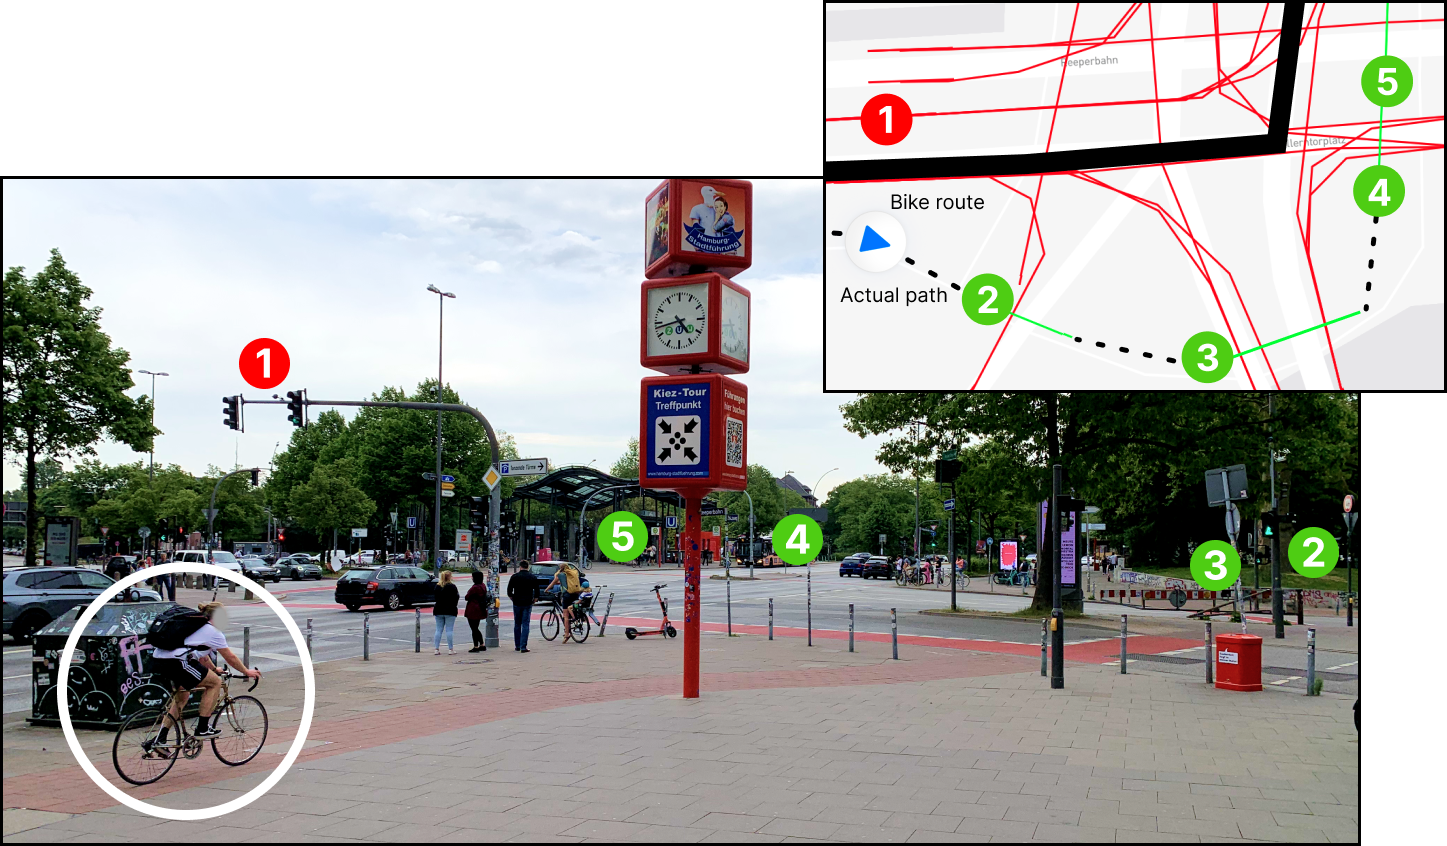
\includegraphics[width=\linewidth]{images/sg-selection-example.png}
\caption{In this case, the OpenStreetMap route does not accurately depict the cyclist's most optimal path and runs over car traffic light 1. In reality, the bike path and four bike/pedestrian traffic lights to the right of the route are utilized: 2, 3, 4, and 5. Source: \cite{matthes2023geo}, [\hyperref[attribution]{Attribution}]}
\label{fig:sg-selection-example}
\end{figure}

As a data foundation for the proposed method, intersection (MAP) topologies provided through the Traffic Lights Data platform are utilized. For each traffic light, a line geometry is given that shapes the lane associated with the traffic light. Which type of traffic is served by the traffic light is also given through the metadata.

Since no precise network graph is available for Hamburg that incorporates both bike paths and traffic light geometries, a different solution must be established to bring together route and traffic light information. In this concept, we will focus on route calculation with publicly available routing foundations such as OpenStreetMap (OSM) and matching the traffic lights along these routes. This solution should then readily apply to other cities as well and has the advantage that we can use the bike path metadata provided through the map foundation later on.

However, one challenge we must solve is that the route geometry and the intersection topologies do not align perfectly. Often, as shown in \Cref{fig:sg-selection-example}, the bike route generated based on OSM utilizes car lanes, although bike lanes are available. It also generally lacks the level of intersection detail required for a direct lookup of nearby traffic lights. Ideally, the matching method should counteract this problem and reasonably decide between the available traffic lights at an intersection in relation to the route geometry. The goal is to replicate a human's intuition by looking at the route's trajectory over the intersection and selecting the correct bike traffic lights using spatial reasoning.

\subsection{Ground Truth and Benchmark}

It is first important to thoroughly understand what a "correct" traffic light means. The correct traffic lights may not always be evident due to the variety of possible intersection traversals depending on contextual circumstances, personal preference, or even spontaneity. Instead, it is about making the most likely selection and then binding the user to this selection through the user interface.

Assuming that cyclists will follow specific movement patterns at each intersection, which are sufficiently predictable by looking at the intersection layout, we can craft examples for optimal selections. As a result, we obtain a ground truth with combinations of routes and traffic lights predicted by a human to match each given route. In the second step, this ground truth can be used to develop and test automated traffic light matching models.

\begin{figure}[t]
\centering
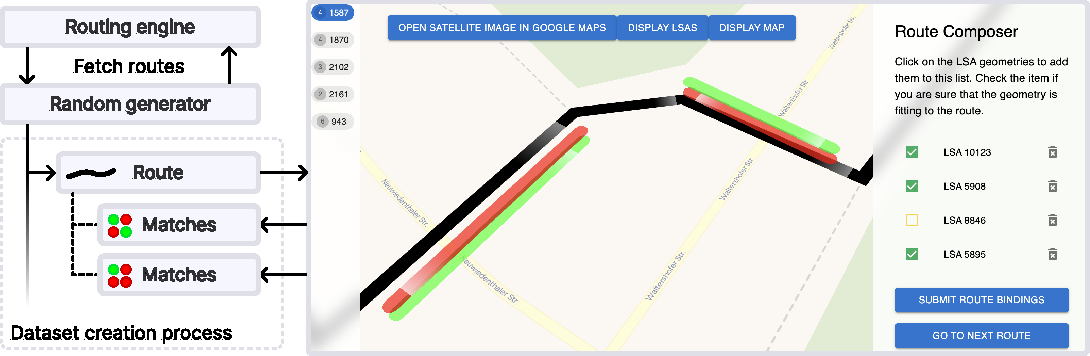
\includegraphics[width=\linewidth]{images/sg-selection-ground-truth.pdf}
\caption{Ground truth creation process through the developed Route Composer app. Sources: \cite{matthes2022matching, matthes2023geo},  [\hyperref[attribution]{Attribution}]}
\label{fig:sg-selection-ground-truth}
\end{figure}

There are multiple options for creating examples for optimal selections of traffic lights. For example, one could physically ride through Hamburg along arbitrary routes and note down the most likely utilized traffic lights. Ideally, however, the ground truth could be generated in a less time-consuming way without the need to travel to Hamburg or any other remote city in which the application is deployed. 

The proposed tool "Route Composer" delivers this possibility. Instead of physically driving through Hamburg, the Route Composer is a web application that allows traveling virtually along randomly generated routes and labeling the correct traffic lights. As shown in \Cref{fig:sg-selection-ground-truth}, the Route Composer highlights the traffic light and route geometries on a map. Then, the traffic lights can be selected by clicking on them in the web application. Once a route is finished, the selected examples are stored for model evaluation.

Independent of how we generate examples for traffic light matching, they may be biased by limited knowledge of the intersection or personal preference, potentially leading to selections that do not represent the most likely choice. To avoid these improper selections as much as possible, two measures are employed: Assuming that the composing is done carefully enough to notice an ambiguous situation, the Route Composer provides the option to open the current intersection in Google Maps for additional cues. The second measure is an explicit ruleset that determines how to handle specific situations:

\begin{enumerate}
\item Consideration is given to traffic flow and the feasibility of safely maneuvering through the intersection.
\item The intersection traversal must be entirely legal according to turn restrictions and street laws.
\item Preference is given to dedicated bicycle lanes or paths indicated by distinct markings or signage.
\item The overall continuity of the route is maintained to ensure a smooth and logical progression.
\item Lanes on the wrong roadside must be avoided.
\item Lanes should never be in an opposing direction to the route.
\end{enumerate}

Based on this ground truth, we can run a benchmark that evaluates the performance of the developed methods. For each route in the ground truth, the matching procedure is executed and produces a list of matched traffic lights. Then, this list of traffic lights is compared to the ground truth, resulting in a number of true negatives, false negatives, true positives, and false positives. Based on these statistics, a benchmark score is calculated.

In selecting the benchmark metric, a few more considerations are required. Since many of the thousands of traffic lights can be excluded entirely by applying a rough distance threshold around the route, many true negatives are expected. These easily excluded traffic lights are not of interest here. What is of interest are the traffic lights near the route for which a more thorough decision is required. Thus, a metric is required that ideally excludes true negatives. The F1 score is chosen here since it only considers true positives (TP), false positives (FP), and false negatives (FN): 

\begin{equation}
\text{\footnotesize F1 Score} = 2 \times \frac{\text{\footnotesize Precision} \times \text{\footnotesize Recall}}{\text{\footnotesize Precision} + \text{\footnotesize Recall}} \quad \text{\footnotesize where} \quad \text{\footnotesize Precision} = \frac{TP}{TP + FP} \quad \text{\footnotesize and} \quad \text{\footnotesize Recall} = \frac{TP}{TP + FN}
\end{equation}

Assuming that especially false-positive or false-negative matches limit the speed advisory's perceived usability, the F1 score is suitable to depict the perceived quality of the matching accurately.

\subsection{Preliminary Approaches}

While exploring potential methods to solve the traffic light matching problem, several methods were tested preliminarily but discarded as they did not perform as well as expected. Before we come to the successful methods for traffic light matching, it is valuable to analyze the failures and learn why these methods did not work as expected. These learnings have been crucial to shaping the final solution, which will be presented afterward.

\subsubsection{H3 Approach}

The H3 approach is based on an idea by colleagues who applied a similar method to cluster inaccurately aligned GNSS paths, obtaining the main directions of intersection traversal and stopping points. The core of this approach is the H3 raster, which subdivides the earth primarily into hexagonal cells\footnote{Strictly speaking, the H3 raster has 12 additional pentagons on every level to complete a seamless shape. See: \url{https://h3geo.org/docs/core-library/restable/}}. On the top resolution level (1), there are 122 cells covering the earth's surface. On level 2, the 122 cells are subdivided into 842 cells, and so forth. As a result, the H3 model contains 15 levels, which are hierarchically connected in a tree structure. This hierarchical structure makes it possible to efficiently navigate through the index, e.g., to find neighbor cells. 

In the work by colleagues, after the GNSS samples of each user track were assigned to an H3 cell, the resulting cells each contained a number of samples and travel direction (edge of the H3 cell), resembling a histogram of the trajectories spatially aligned with the intersections. Assuming a normally distributed GNSS scattering around the actual position, the buckets could then be used to sift out the most frequently used pathways of cyclists statistically. Minor GNSS errors or individualities in the user movement do not fall into weight as they are clustered together. Since this approach was described as remarkably successful, the fundamental idea was further explored to identify potential methods for aligning the traffic light geometries with the inaccurate bike route.

\begin{figure}[t]
\centering
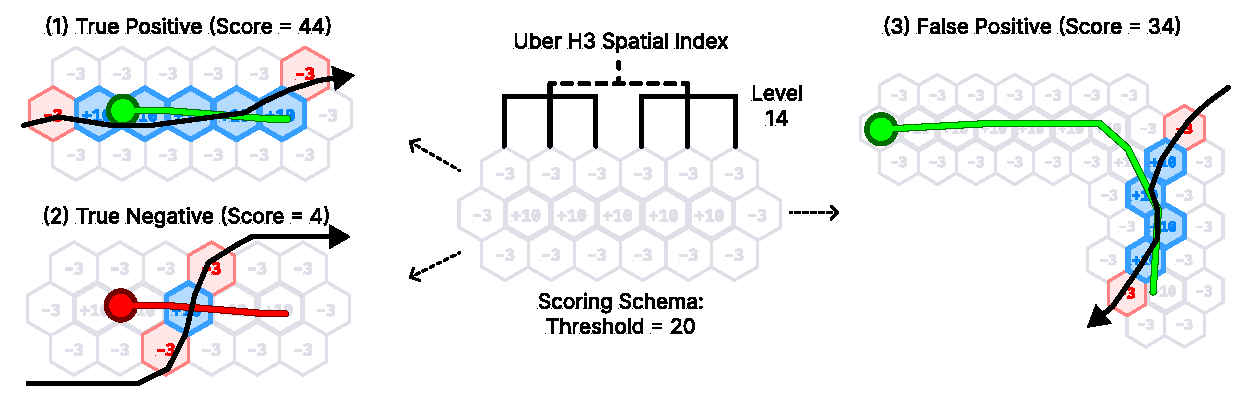
\includegraphics[width=\linewidth]{images/sg-selection-h3-approach.pdf}
\caption{Illustration of the matching procedure behind the developed H3 approach.}
\label{fig:sg-selection-h3-approach}
\end{figure}

The initial idea was to count the cells aligned between route geometry and traffic light geometries. The traffic light is detected as a match if sufficient overlap is found. After testing multiple H3 levels, the H3 level 14 was determined empirically to provide the best tradeoff between resolution and tolerance to imperfect alignment. To emphasize the importance of a near-parallel alignment, a ring-based scoring schema as illustrated in \Cref{fig:sg-selection-h3-approach} was tested that penalizes crossing geometries (2) and favors parallel-aligned geometries (1). This ring-based scoring schema uses H3's tree structure to find neighboring cells of the traffic light geometry efficiently.

Nonetheless, a significant challenge is finding a suitable scoring threshold for the number of matched cells until a traffic light is counted as a "match." Some traffic light geometries may be only a few meters long, while others are much longer. Since longer geometries contain more cells, it is more likely that these are false-positively matched to the route, while short geometries often produce false negatives. After testing multiple different scoring schemas and thresholds and coming to the final scoring schema highlighted in \Cref{fig:sg-selection-h3-approach}, achieving a sufficiently good matching was impossible. In the developed benchmark, an F1 score of 50\% was never exceeded. 

One identified improvement possibility was applying a relative scoring schema for each traffic light. Instead of applying absolute values to each H3 cell around the line geometry, the scoring schema would be scaled inversely proportional to the number of cells. This means a longer line geometry would have more cells with lower individual scores than a short geometry. Ideally, the result would be a normalized alignment score for each traffic light geometry that can be subjected to a universal threshold. Figuratively, the score would depict how much both geometries align. However, this potential solution was not thoroughly explored due to other systematic limitations of the H3 approach.

\begin{figure}[t]
\centering
\frame{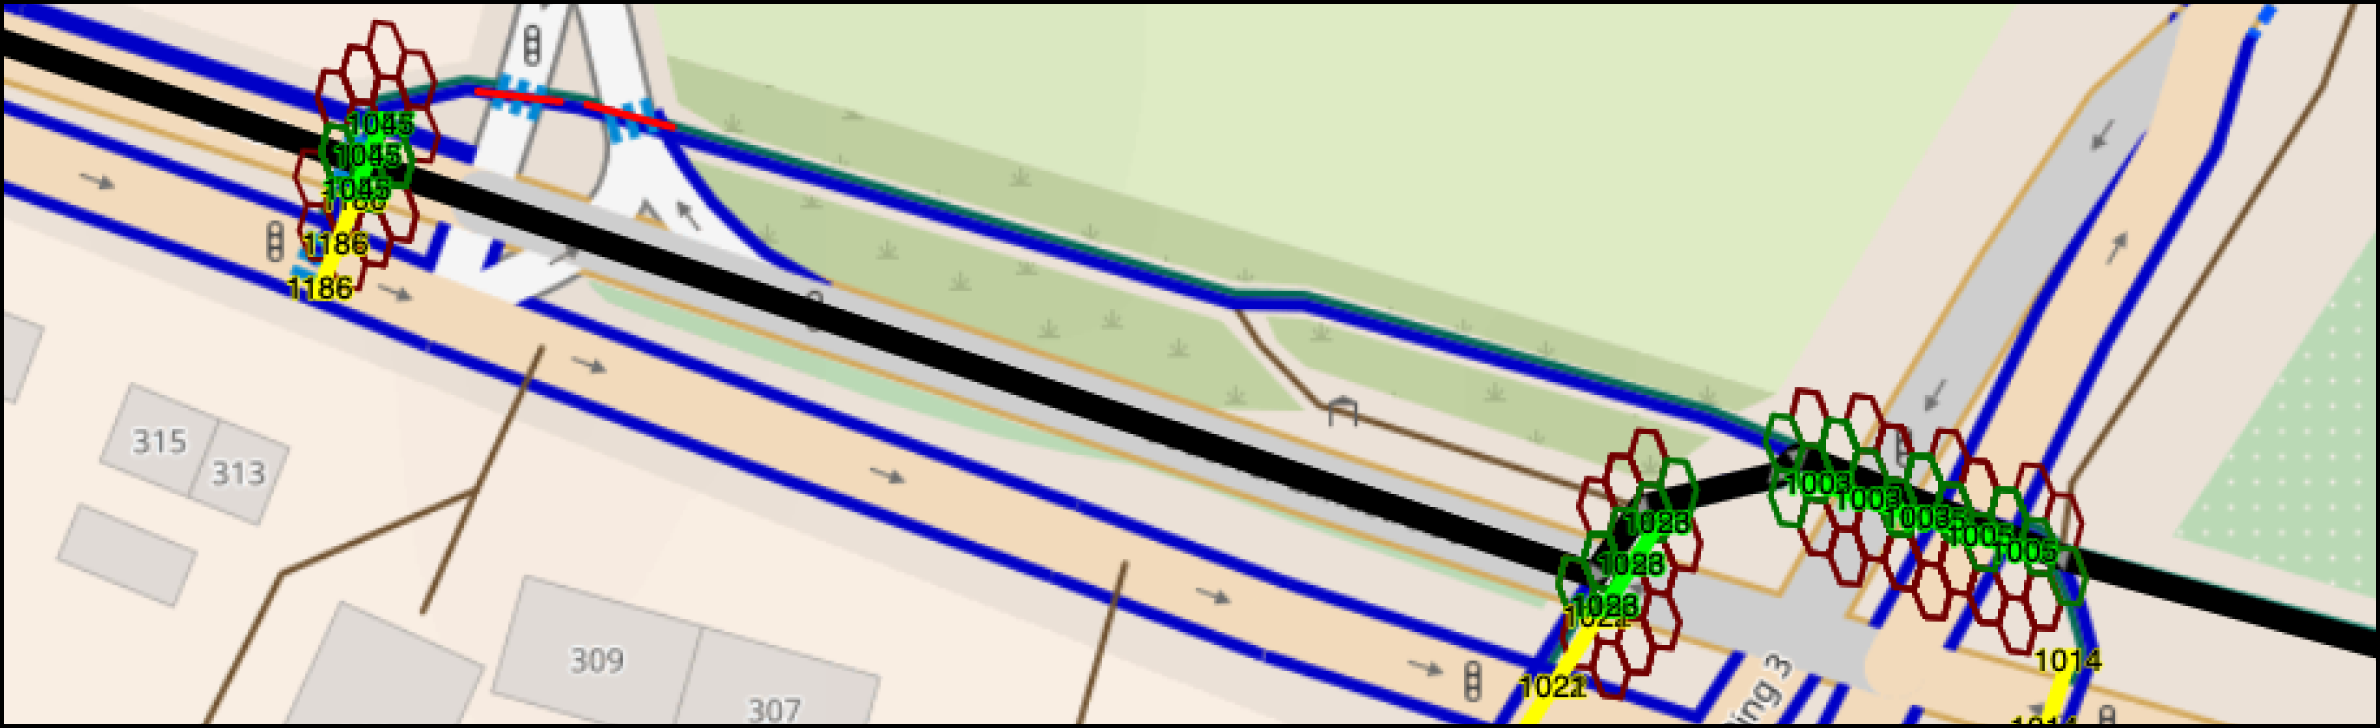
\includegraphics[width=\linewidth]{images/sg-selection-h3-example.png}}
\caption{Example of four traffic lights matched using the H3 approach along the route. [\hyperref[attribution]{Attribution}]}
\label{fig:sg-selection-h3-example}
\end{figure}

The main limitation of the H3 approach is that it assumes that the route geometry is near enough to the matching traffic light geometries. However, considering OSM's mixed coverage of bike paths, many false negatives were produced when the route was mapped on the car lanes while the appropriate bike traffic light was located on the bike path a few meters to the side of the road. 

A potential solution to this problem would be to choose a larger raster, which would worsen the score even more since many traffic lights' geometries are no longer captured adequately. Instead, they would resemble a circular "blob," as highlighted on the left side of \Cref{fig:sg-selection-h3-example}. The "blob" problem does not only appear when upscaling the raster to H3 level 13. It appears at level 14 as well. Some traffic lights would have such short geometries that only one H3 cell was matched, especially concerning pedestrian traffic lights crossing the road. Since many of these traffic lights are aligned orthogonally to the road's direction, the loss of the traffic light's direction information in the "blob"-shaped scoring schema would ultimately lead to erroneous matchings. Increasing the resolution level to 15 would mitigate this problem and introduce a more shaped raster around the line geometries. However, it would again increase the volatility against offset traffic lights along the route.

Due to these issues, the H3-based approach for traffic light matching was not further explored. The takeaway from this approach is that close alignment does not sufficiently model matching traffic lights along a route geometry. Instead, the traffic light geometries may sometimes be offset from the route, especially if the route is snapped onto the car lanes.

\subsubsection{Graph Approach}

The second approach is inspired by the map-matching procedure proposed by Newson and Krumm in 2009 \cite{newson_hidden_2009}. Their proposed method matches GNSS trajectories to the road network by building a transition graph between each GNSS sample and the nearby roads. After the graph is created, each transition is marked with a transition probability. Their approach calculates the most probable path through the transitions using the Viterbi algorithm to find the most likely sequence of roads taken. The idea was to transfer this approach to traffic light matching, interpreting the route geometry as GNSS trajectory and the traffic light geometries as road segments.

\begin{figure}[t]
\centering
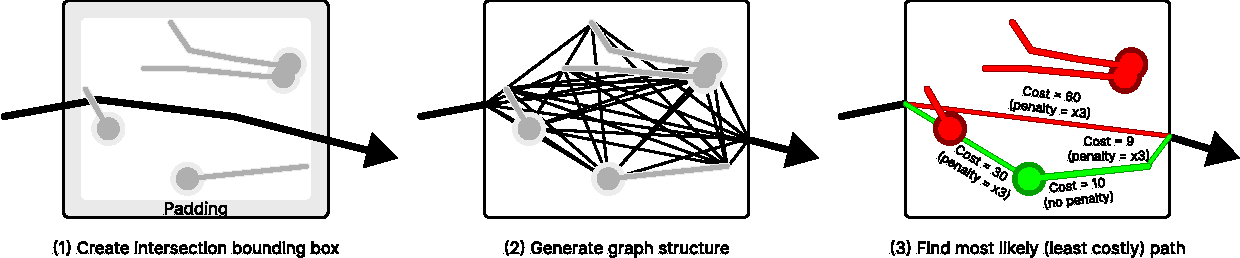
\includegraphics[width=\linewidth]{images/sg-selection-graph-approach.pdf}
\caption{Steps for traffic light matching in the graph-based approach.}
\label{fig:sg-selection-graph-approach}
\end{figure}

The proposed approach operates as illustrated in \Cref{fig:sg-selection-graph-approach}. First, traffic lights along the route are prefiltered using a rough distance threshold of 20m. The remaining traffic lights are clustered into intersections based on the intersection node ID. The procedure undergoes three steps around these intersections: (1) A bounding box is calculated with an additional padding. The route enters and exits the bounding box at one point. (2) A fully connected graph is generated between the route's entry and exit points and each traffic light geometry's start and end points. (3) A cost is assigned to each transition in the graph based on the transition's length. Finally, the least costly path is calculated using the Dijkstra pathfinding algorithm. This path should then represent the most likely utilized trajectory over the traffic light geometries.

The cost function is defined to penalize traversal between traffic lights, and traversal using the traffic lights is preferred. Otherwise, the most optimal path would always be the direct connection between the entry and exit points. Specifically, every transition in the graph  $(p_{1} \rightarrow p_{2})$ has the cost $dist(p_{1}, p_{2})$, while transitions between traffic lights have the cost $dist(p_{1}, p_{2}) \times \text{penalty}$. Thus, the penalty value represents a hyperparameter of the model together with the dimensions of the intersection padding. 

Which penalty value and intersection padding to choose may depend on each intersection's characteristics. Thus, defining these hyperparameters by hand would not be the best option. A better option is to utilize a tuning algorithm that automatically approximates the optimal configuration based on the developed ground truth. Specifically, the Tree-Structured Parzen Estimator hyperparameter tuning algorithm is utilized \cite{ozaki_multiobjective_2020}. This tuner considers each hyperparameter (intersection padding and penalty) independently from each other. During the tuning, the model undergoes inference for all routes in the dataset (one trial). After each trial, the F1 score is evaluated, and the tuner adjusts the hyperparameters into a direction estimated to result in a better score.

\begin{figure}[t]
\centering
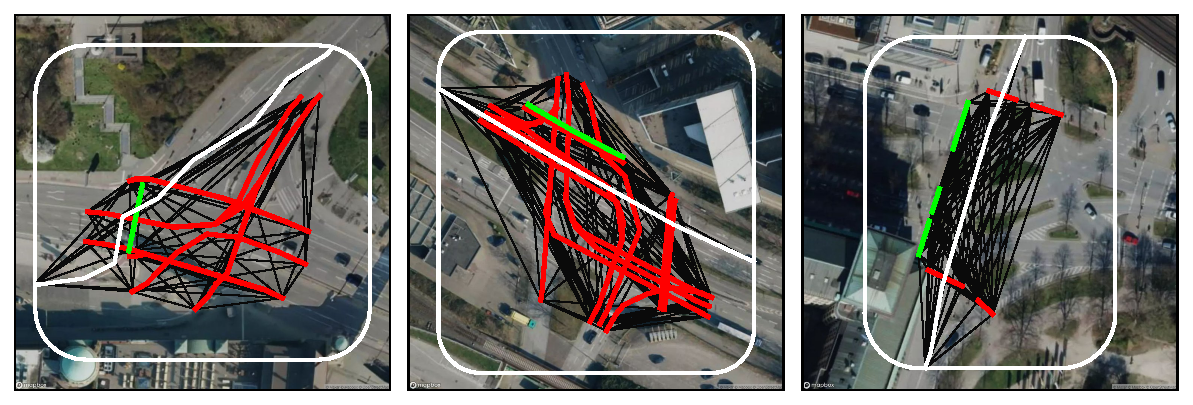
\includegraphics[width=\linewidth]{images/matching-dijkstra-correct.pdf}
\caption{Examples of correct matching using the graph approach. [\hyperref[attribution]{Attribution}]}
\label{fig:sg-selection-graph-example}
\end{figure}

After tuning the model to the ground truth, the model reached an F1 score of 75.4\% (penalty = 2.87, padding = 25m). As a distance function, this version of the model utilizes the Euclidean distance between the coordinates in the WGS84 projection system. Correct matchings from this model highlighted in \Cref{fig:sg-selection-graph-example} indicate the model's capabilities. The model would perform well even in scenarios where the traffic light's geometry is offset to the route and thus has considerable advantages over the H3 approach, as reflected in the improved F1 score.

\begin{figure}[t]
\centering
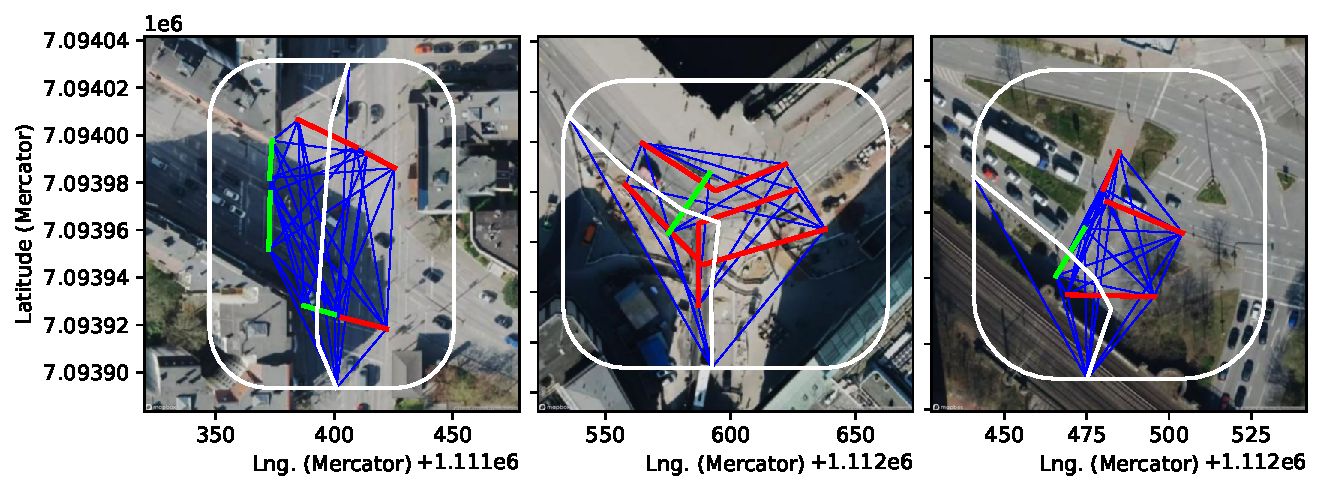
\includegraphics[width=\linewidth]{images/matching-dijkstra-incorrect.pdf}
\caption{Examples of false matching using the graph approach. [\hyperref[attribution]{Attribution}]}
\label{fig:sg-selection-graph-fails}
\end{figure}

However, the final result is still not convincing, considering that the measured score of 75.4\% represents a training F1 score and was not evaluated on unseen data. By studying many error cases, one particular weakness was identified. As highlighted in \Cref{fig:sg-selection-graph-fails}, the model would struggle particularly with right or left turns at intersections. In these cases, the route exits the bounding box adjacent to the ingress's edge. In these cases, the direct distance from the ingress point to the egress point is often lower than the path over the correct traffic lights' geometries. As a result, the model tends to shortcut directly to the intersection exit. Two solutions are possible to address these cases:

\begin{enumerate}
    \item Increasing the penalty for traveling off a traffic light's geometry. A separate penalty could be applied in cases where the ingress and egress edges of the bounding box are adjacent to avoid shortcuts.
    \item  Modifying the graph generation procedure to strictly "go back" to the nearest point on the route after each traversal of a traffic light's geometry. Thus, the penalty for attempted shortcuts (going off the route) would increase drastically.
\end{enumerate}

Option one initially may seem like a good choice here. However, this strategy would worsen another problem highlighted in \Cref{fig:sg-selection-graph-fails}: traffic light geometries are often falsely traversed because their exit point is slightly more proximal to the egress point. A higher penalty amplifies this problem. Thus, option two was implemented instead. 

Unfortunately, the adjusted graph generation procedure's result is a worse F1 score after hyperparameter tuning of 60.7\% (penalty = 9.68, intersection padding = 42m). In many cases, the model would now avoid shortcutting as intended, but the model would also be noticeably more strict. The reason is that the traffic lights' geometries are no longer connected but rather through the route (see \Cref{fig:sg-selection-graph-strict}). Jumping on and off the traffic light geometries would often be a worse option for the pathfinding algorithm than staying on the route, even with a remarkably higher penalty. 

Another variation of the graph-based approach would be to cut out the intersections, reconnect the OSM paths via the traffic light geometries, and then calculate the route using these. However, the main problems here are similar, especially the problem of connecting the traffic light geometries and the problem of stitching at the edges. Thus, this idea was not further explored.

\begin{figure}[t]
\centering
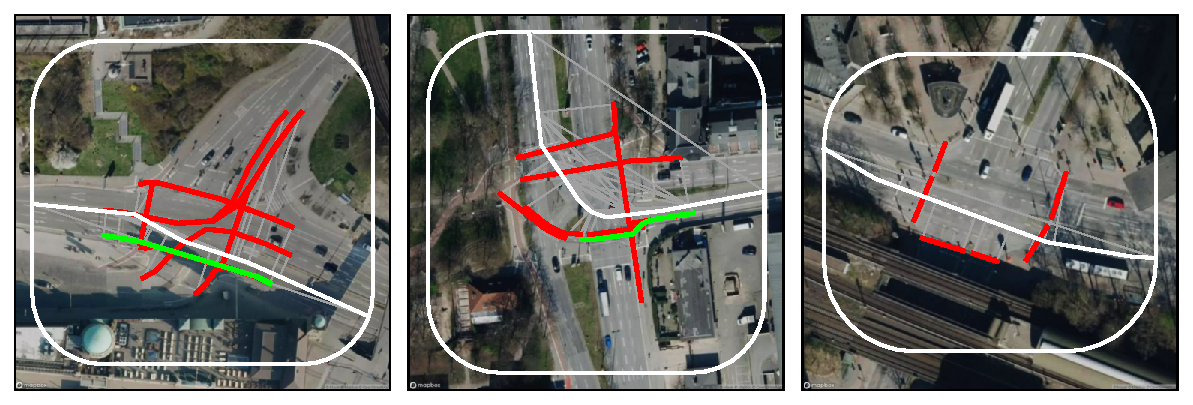
\includegraphics[width=\linewidth]{images/matching-dijkstra-strict.pdf}
\caption{Examples of matching using the adjusted graph generation procedure. [\hyperref[attribution]{Attribution}]}
\label{fig:sg-selection-graph-strict}
\end{figure}

Although the developed graph-based methods initially promised good results, they were ultimately not further studied in favor of more promising ideas. Even if the graph approach seems less susceptible to offsets and longer traffic light geometries, it falls short when considering the curvature and not only the absolute location of the traffic light geometries. In the end, only the start and end points of each traffic light geometry are considered. However, the curvature is similarly essential to decide which traffic light could match the associated route.

\subsubsection{Map-Matching Approach}

A positive learning of the graph-based approach is that the map-matching problem of Newson and Krumm (2009) \cite{newson_hidden_2009} is, in theory, very similar to the problem we are trying to solve. Another idea based on this approach would be to map-match the traffic light geometries onto the OSM road network, fusing both map sources and allowing for a direct traffic light lookup.

\begin{figure}[b]
\centering
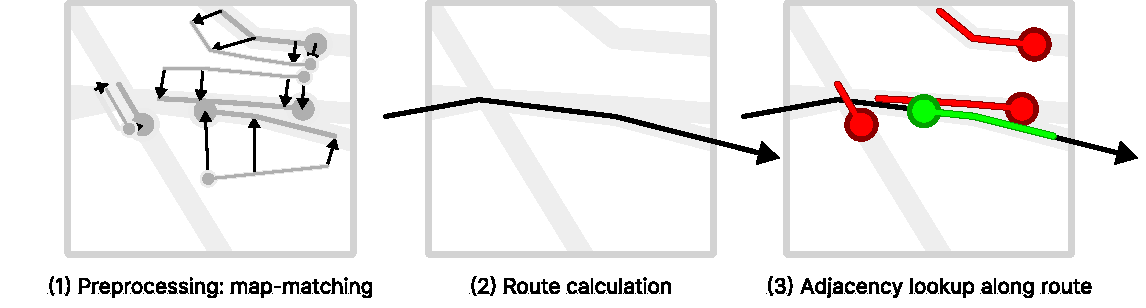
\includegraphics[width=\linewidth]{images/sg-selection-map-matching-approach.pdf}
\caption{Steps for map-matching traffic lights onto the routing foundation.}
\label{fig:sg-selection-map-matching-approach}
\end{figure}

\Cref{fig:sg-selection-map-matching-approach} illustrates the proposed procedure, consisting of three steps: (1) In a preprocessing step, the traffic light geometries are map-matched onto the routing foundation. As a result, the traffic light geometries align with the routing foundation's topology. (2) The route is calculated using the same routing foundation. (3) All traffic lights that perfectly align with the route's geometry are matched.

The approach by Newson and Krumm (2009) \cite{newson_hidden_2009} is utilized as a map-matching procedure. This approach is implemented by default in the GraphHopper routing engine and can be accessed through its map-matching API\footnote{\url{https://docs.graphhopper.com/\#tag/Map-Matching-API}}. Each traffic light geometry is transformed into a compatible format (GPX) and sent to the map-matching API, which projects the geometry onto the integrated routing foundation (OpenStreetMap).

\begin{figure}[t]
\centering
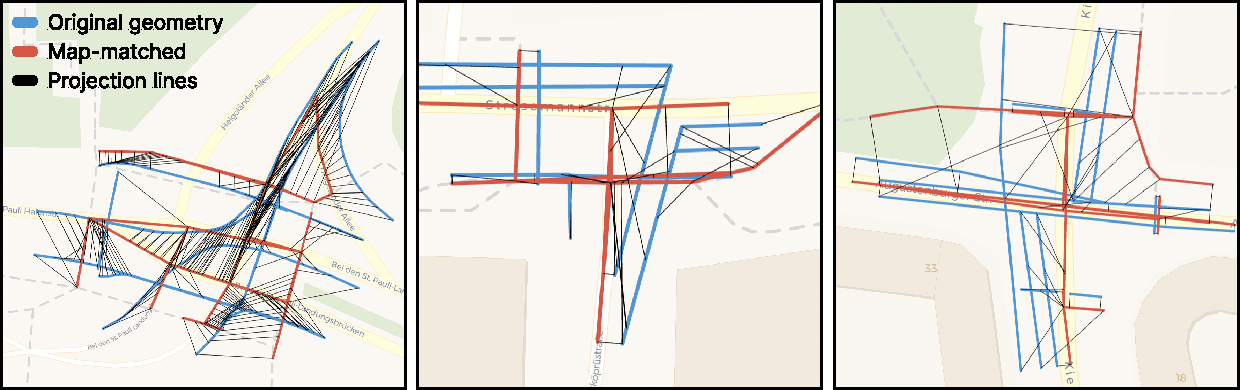
\includegraphics[width=\linewidth]{images/sg-selection-map-matching-fails.pdf}
\caption{Distortion of traffic light geometries after map-matching. [\hyperref[attribution]{Attribution}]}
\label{fig:sg-selection-map-matching-fails}
\end{figure}

Despite the promising idea, when testing the approach with the OSM routing foundation, a substantial problem was determined. Although it was possible to project the traffic light geometries onto the routing foundation, they were distorted entirely during the process. Examples of this distortion are highlighted in \Cref{fig:sg-selection-map-matching-fails}. These distortions may be amplified by the problem that traffic light geometries are usually shorter than typical GNSS trajectories for which the map-matching approach was initially conceived. Without enough intersection detail in the routing foundation, the map-matching procedure often seems to fail to find a suitable projection. Moreover, multiple traffic lights may be matched onto the same path segment, resulting in an ambiguous matching. 

Since not only bike traffic lights are represented in the system but also traffic lights shared between cars/buses and bikes, this approach would require a routing foundation that represents all of the respective paths (not only bike paths) noticeably more accurately than OSM, such as a multimodal HD map. Whether this approach applies to such a map could not be tested as none was available. Due to these findings, the map-matching method was also not investigated further.

\subsection{Algorithmic Filtering Approach}

The preliminary H3, graph, and map-matching approaches have not been successful but provided a deeper understanding of the problem. First, an ideal matching procedure should be robust against offsets of the traffic light geometries from the route, especially when the route geometry is mapped on the road while the bike traffic light is alongside. Second, the matching procedure must handle long and short traffic light geometries. 

\begin{figure}[t]
\centering
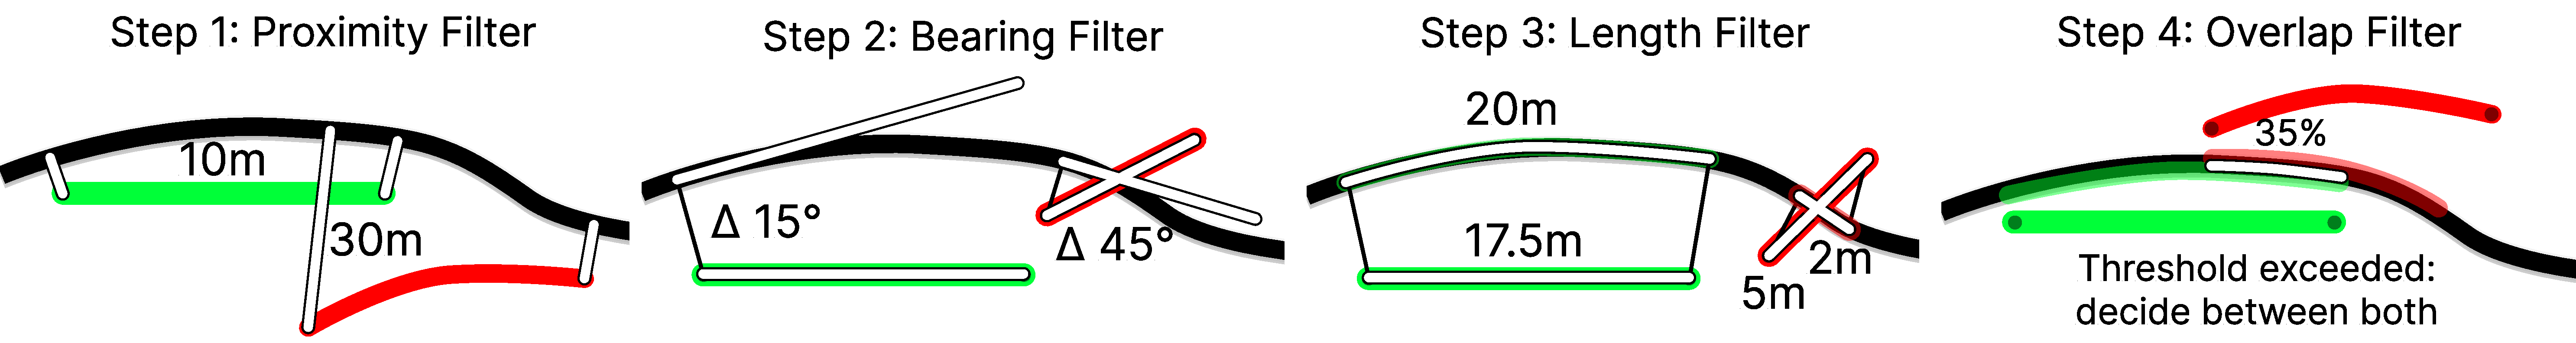
\includegraphics[width=\linewidth]{images/sg-matching-filters.pdf}
\caption{Filtering steps for matching with the algorithmic approach.}
\label{fig:sg-matching-filters}
\end{figure}

Most importantly, it is crucial to consider the absolute location of the traffic light geometries along the route and their geometrical properties in relation to the route. If the traffic light's geometry is aligned near the route and follows its curvature, it will likely match the route. The question is how to model this relation and tell apart edge cases mathematically.

One solution is to tell apart matching from non-matching traffic light geometries by comparing their shapes with the route. In four filtering steps, specific geometric thresholds are applied to filter out traffic lights that are likely no match. The idea is that each step catches a specific type of misalignment with the route, such that, in the end, only the wanted matches remain. As shown in \Cref{fig:sg-matching-filters}, four filtering steps are employed: proximity filter, bearing filter, length filter, and overlap filter.

\textbf{\color{cidarkblue}Step 1 -- Distance Filter:} Step one focuses on coarsely excluding a large proportion of the traffic lights in the city area through a distance threshold $t_{dist}$ from the route. This step is efficiently executed through a PostGIS database using the \texttt{ST\_Distance}\footnote{\url{https://postgis.net/docs/en/ST\_Distance.html}} query.

\textbf{\color{cidarkblue}Step 2 -- Bearing Filter:} As a next step, the bearing between the traffic light's geometry and the route is compared. As a result of this, we can exclude traffic lights that are angled too steeply or even inverted to the route. As a foundation, the atan2 function is used to calculate the bearing between two coordinates on the earth\footnote{\url{https://www.movable-type.co.uk/scripts/latlong.html}}:

\begin{equation}
x(c_1, c_2) = sin(lon_2 - lon_1) \times cos(lat_2)
\end{equation}
\begin{equation}
y(c_1, c_2) = cos(lat_1) \times sin(lat_2) - (sin(lat_1) \times cos(lat_2) \times cos(lon_2 - lon_1))
\end{equation}
\begin{equation}
bear(c_1, c_2) = atan2(x(c_1, c_2), y(c_1, c_2))
\end{equation}

where $c_1 = (lat_1, lng_1)$ and $c_2 = (lat_2, lng_2)$ are WGS84 coordinates (in radians). As a result, we can calculate the bearing of the traffic light's geometry $(c_1, \dots, c_n)$ based on its first two coordinates. To compare this bearing to the route geometry, the traffic light geometry is projected onto the route. Every coordinate $(c_1, \dots, c_n)$ is mapped to the nearest point on the route geometry $(\bar{c_1}, \dots, \bar{c_n})$. Then, the bearing diff $\bar{\Delta}_{bear_1}$ is calculated as:

\begin{equation}
    \bar{\Delta}_{bear_{i=1}} = 
        abs(\underbrace{bear(c_{i=1}, c_{i+1=2})}_{\text{Bearing of traffic light geometry}} - \underbrace{bear(\bar{c}_{i=1}, \bar{c}_{i+1=2})}_{\text{Bearing of projection on route}})
\end{equation}

The bearing diff $\bar{\Delta}_{bear_1}$ denotes how much the traffic light's angle differs from the route's at the nearest point to the first traffic light geometry coordinate. The calculated value can be subjected to a bearing threshold $t_{bear}$, which defines if the traffic light's geometry is counted as a match or not:

\begin{equation}
\Psi_{bear_{i=1}} = 
    \begin{cases}
            1,& \text{if } \bar{\Delta}_{bear_{i=1}} \in \left(-t_{bear}, t_{bear}\right)\\
            0,              & \text{otherwise}
        \end{cases}
\end{equation}

where $\Psi_{bear_{i=1}} = 1$ means that the segment is angled similarly enough to the nearby route and is considered a match. All traffic lights that are not a match ($\Psi_{bear_{i=1}} = 0$) are filtered out. For example, if $t_{bear} = 45^{\circ}$, we will filter out all geometries whose first coordinate is angled more than $\pm 45^{\circ}$ relative to the projection onto the route. 

\begin{figure}[b]
\centering
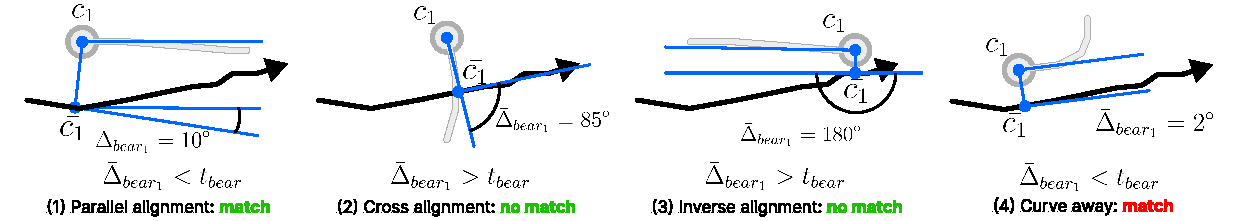
\includegraphics[width=\linewidth]{images/sg-selection-bearing-filter.pdf}
\caption{Examples for bearing matching based on traffic light geometry's first coordinate.}
\label{fig:sg-selection-bearing-filter}
\end{figure}

This process is drawn in \Cref{fig:sg-selection-bearing-filter}. In cases (1), (2), and (3), the alignment of both geometries is classified correctly. However, (4) illustrates one particular weakness: traffic light geometries initially aligned but then curving away from the route are not filtered out correctly. The reason is that only the first coordinate is compared, not the complete geometry. To compare the complete geometry, all coordinates $c_i$ of the traffic light geometry are compared to the route. Then, a weighted sum $\phi_{bear}$ is calculated, incorporating the length of each geometry segment relative to the complete geometry. In this way, longer parts of the traffic light's geometry are emphasized:

\begin{equation} 
\phi_{bear} = 
    \underbrace{\sum_{i=1}^{n-1} 
    \frac{\Psi_{bear_i}}{dist(c_i, c_{i+1})}}_{\text{Sum of matching segment lengths}}
    \times
    \underbrace{(\sum_{i=1}^{n-1} dist(c_i, c_{i+1}))^{-1}}_{\text{Sum of segment lengths}}
\end{equation}

where $dist$ is calculated as the Euclidean distance and $n$ is the number of coordinates in the traffic light's geometry. As a result, $\phi_{bear}$ is normalized between 0 and 1. $\phi_{bear} = 0$ means none of the traffic light geometry's segments matches the angular threshold $t_{bear}$, while a value of 1 represents a full match. To determine the decision boundary between match and no match, $\phi_{bear}$ is subjected to another threshold $t_{bear\_sum} \in [0, 1]$. This threshold is chosen to exclude traffic lights curving away from the route.

\begin{figure}[b]
\centering
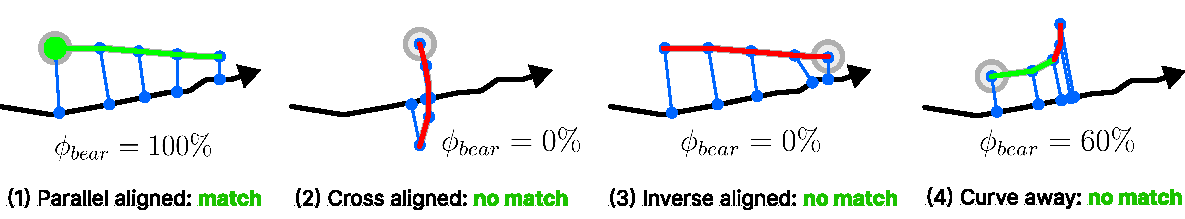
\includegraphics[width=\linewidth]{images/sg-selection-bearing-filter-sum.pdf}
\caption{Examples for (cumulative) bearing matching.}
\label{fig:sg-selection-bearing-filter-sum}
\end{figure}

\Cref{fig:sg-selection-bearing-filter-sum} gives an intuition for the final working principle of the bearing filter. In example (1), all the traffic light's geometry segments are sufficiently aligned to the route. Examples (2) and (3) depict cases where none of the segments are within the angular threshold $t_{bear}$. Example (4) highlights a case where the first 60\% of the traffic light geometry matches the route. In the illustration, $t_{bear\_sum}$ is assumed to be larger than 60\%, so the traffic light that curves away is filtered out. The higher this threshold is configured, the more aggressively the filter excludes inclined geometries.

\textbf{\color{cidarkblue}Step 3 -- Length Filter:} With the previous two steps, we have two bearing thresholds ($t_{bear}$ and $t_{bear\_sum}$) in addition to the distance threshold $t_{dist}$. However, during the systematic testing of the thresholds, it quickly became apparent that they alone cannot sufficiently distinguish matching traffic lights from non-matching traffic lights. A key observation was made during the search for other characteristics that distinguish matching from non-matching traffic lights: Non-matching traffic light geometries often have a shorter projection onto the route relative to their original length. This feature is also related to the traffic light geometry's angular position to the route but incorporates the shape of the route in between projected traffic light geometry coordinates.

\begin{figure}[t]
\centering
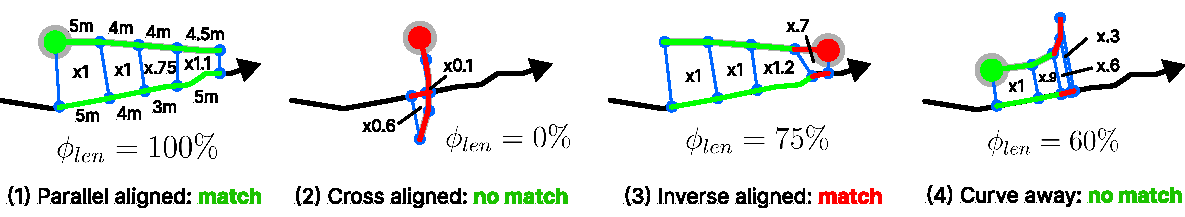
\includegraphics[width=\linewidth]{images/sg-selection-length-filter-sum.pdf}
\caption{Examples for (cumulative) length matching.}
\label{fig:sg-selection-length-filter-sum}
\end{figure}

To mathematically represent this intuition, a cumulative score $\phi_{len}$ is calculated similarly to the bearing filter and then subjected to a threshold $t_{len\_sum}$. The score $\phi_{len}$ quantifies the difference from 0 (no matching segments) to 1 (all segments matching), again weighted by the length of each segment. Example (3) shows that the length filter does not detect inversely aligned geometries well. However, since the bearing filter is assumed to handle this case, the length filter will likely not encounter such constellations.

Due to the similarity with the bearing filter, we can reuse its formulas and only have to replace the metric $\Psi$, which determines whether a segment is counted as a match. First, each segment $(c_1, \dots, c_n)$ is again projected onto the route as $(\bar{c_1}, \dots, \bar{c_n})$. Then, the length diff $\bar{\Delta}_{len_1}$ for the i-th segment is calculated as:

\begin{equation}
    \bar{\Delta}_{len_i} = 
        \begin{cases}
            0,& \text{if } line\_dist(\bar{c}_i, \bar{c}_{i+1}) = 0 \\
            abs(\frac{dist(c_{i}, c_{i+1})}{line\_dist(\bar{c}_{i}, \bar{c}_{i+1})}),              & \text{otherwise}
        \end{cases}
\end{equation}

where $dist$ is calculated as the Euclidean distance, and $line\_dist(\bar{c}_i, \bar{c}_{i+1})$ represents the distance along the route's geometry between $\bar{c}_i$ and $\bar{c}_{i+1}$. To calculate $line\_dist$, it is necessary to interpolate along the route's geometry. Using the calculated length diff, each segment of the traffic light's geometry is mapped as:

\begin{equation}
\Psi_{len_i} = 
    \begin{cases}
            1,& \text{if } \bar{\Delta}_{len_{i}} \in \left(1 - t_{len}, 1 + t_{len}\right)\\
            0,              & \text{otherwise}
        \end{cases}
\end{equation}

where $\Psi_{len_i} = 1$ means the segment matches the length diff threshold $t_{len}$. Finally, the weighted sum of all traffic light geometry segments is calculated as follows:

\begin{equation} 
\phi_{len} = 
    \underbrace{\sum_{i=1}^{n-1} 
    \frac{\Psi_{len_i}}{dist(c_i, c_{i+1})}}_{\text{Sum of matching segment lengths}}
    \times
    \underbrace{(\sum_{i=1}^{n-1} dist(c_i, c_{i+1}))^{-1}}_{\text{Sum of segment lengths}}
\end{equation}

Here, $\phi_{len} = 0$ means that all of the traffic light geometry's segments are shortened too much when projecting them onto the route geometry, indicating a traffic light that is not aligned with the route. Likewise, $\phi_{len} = 1$ means that all segments roughly stay the same length when projected onto the route. To distinguish when a traffic light is counted as a match, the thresholds $t_{len}$ and $t_{len\_sum}$ can be optimized accordingly.

\textbf{\color{cidarkblue}Step 4 -- Overlap Matcher:} The previous matching steps often struggle with one particular problem: multiple parallel-aligned traffic lights. Often, this case leads to a multi-selection of these traffic lights, while only one of them will be taken by the cyclist. On the other hand, especially on complex intersections, there may be multiple consecutive traffic lights whose geometries partially overlap along the route but are still a valid match. Thus, some overlaps must be filtered out, while others are intentional.

\begin{figure}[b]
\centering
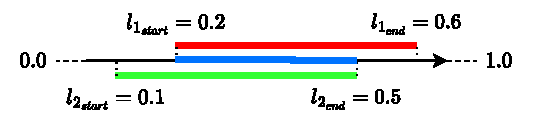
\includegraphics[width=0.5\linewidth]{images/overlap.drawio.pdf}
\caption{Example overlap.}
\label{fig:sg-matching-overlap-filter}
\end{figure}

First, the overlaps between traffic lights with respect to the route are determined. To accomplish this, the traffic lights' geometries are snapped onto the route. As a result, each traffic light's start and end points along the route are determined, as highlighted in \Cref{fig:sg-matching-overlap-filter}. For each pair of matched traffic light geometries $(l_1, l_2)$, an overlap percentage $\phi_{overlap}$ is calculated as:

\begin{equation}
    \phi_{overlap} = \frac{min(l_{1_{end}}, l_{2_{end}}) - max(l_{1_{start}}, l_{2_{start}})}{max(l_{1_{end}}, l_{2_{end}}) - min(l_{1_{start}}, l_{2_{start}})}
\end{equation}

In the error case that the denominator is zero, $\phi_{overlap}$ is also mapped to zero. As soon as this percentage exceeds a threshold $t_{overlap\_pct}$, a decision process between both geometries is initiated:

\begin{enumerate}
    \item According to the traffic light metadata, if one of the traffic lights is a dedicated bike traffic light, choose that one.
    \item If one of both traffic lights perfectly matches the route, select that one. To determine whether a traffic light perfectly matches the route, a distance threshold $t_{perfect\_match}$ is configured.
    \item If both traffic lights are on different sides of the route and the distance between both traffic lights is smaller than a threshold $t_{road\_side}$, prefer the ordinary traffic side (in Germany, right-hand traffic). Whether a traffic light is left or right from the route is determined through $\bar{\Delta}_{bear_{i=1}}$.
    \item Otherwise, decide purely by the distance to the route.
\end{enumerate}

The thresholds $t_{overlap\_pct}$, $t_{perfect\_match}$, and $t_{road\_side}$ can be used to tune the final result. In the case of $\phi_{overlap} < t_{overlap\_pct}$, both traffic lights are kept. This threshold allows for intentional small overlaps at complex intersections without filtering consecutive traffic lights out.

\begin{table}[!b]
\caption{Summary of thresholds and search space.}
\begin{tabular}{@{}lp{8cm}l@{}}
\toprule
\textbf{Hyperparameter}  & \textbf{Explanation} & \textbf{Search Interval} \\
\midrule
T1 ($t_{dist}$) & Traffic light geometries must be within this distance of the route. & $[1m, 100m]$ \\
T2 ($t_{bear\_sum}$) & The minimum proportion of the traffic light's geometry matching $t_{bear}$. & $[0, 100\%]$ \\
T3 ($t_{bear}$) & If segments of the traffic light geometry are angled more steeply to the route than this value, they are not counted for $t_{bear\_sum}$. & $[0^{\circ}, 180^{\circ}]$ \\
T4 ($t_{inv}$) & Whether inverted traffic light geometries should be matched. & $[\text{False}, \text{True}]$ \\
T5 ($t_{len\_sum}$) & The minimum proportion of the traffic light's geometry matching $t_{len}$. & $[0, 100\%]$ \\
T6 ($t_{len}$) & If segments of the traffic light geometry are elongated or shortened more than $1 \pm t_{len}$ when projected onto the route, they are not counted for $t_{len\_sum}$. & $[0, 1]$\\
T7 ($t_{road\_side}$) & If two overlapping traffic lights are on opposite sides of the route and less than this distance away, decide by the ordinary traffic side. & $[0, 100m]$ \\
T8 ($t_{perfect\_match}$) & If a traffic light's geometry is closer to the route than this value, it is preferred over another overlapping traffic light geometry. & $[0, 50m]$ \\
T9 ($t_{overlap\_pct}$) & If two traffic lights overlap more relative to their combined length, a decision process between both traffic lights is initiated. & $[0, 100\%]$ \\
\bottomrule
\end{tabular}
\label{tab:hyperparameter-space}
\end{table}

\paragraph{Model Finetuning:} The designed filtering pipeline has several thresholds that must be carefully selected to optimize the final matching performance. Here, it is essential to consider that each filter influences the subsequent filters in the pipeline. This complexity means tuning the individual filters by hand is challenging and time-intensive. A solution to this problem is utilizing a hyperparameter tuning algorithm, which tries to understand the influence of each hyperparameter on a model and maximizes its score. This algorithm can run overnight, resulting in a proposed model configuration after a few hundred to thousand trials. To prepare the model for hyperparameter tuning, search spaces for each hyperparameter must be defined. These search spaces are summarized in \Cref{tab:hyperparameter-space}. The Tree-Structured Parzen Estimator hyperparameter tuning algorithm \cite{ozaki_multiobjective_2020} is utilized to find a suitable configuration on the ground truth benchmark. The objective function given to the tuner algorithm is the F1 score.

\subsection{Machine Learning Filtering Approach}

One identified problem of the algorithmic approach is that each threshold is defined globally and equally applied to all situations. However, not all intersections are crossed similarly by routes. Thus, the filtering pipeline would be applied too strictly in some situations, while the thresholds are not applied strictly enough in others. Here, an ML model can be useful to employ a more flexible and interlinked mapping of the geometric properties. After this opportunity was identified, such an ML model was investigated under supervision in Daniel Jeschor's Master thesis \cite{jeschor_2022}. The following concepts for the ML approach are based on this thesis.

Regarding the problem of deciding between "match" and "no match" for each traffic light geometry, there may be many creative ways to establish an ML classifier. For example, it would be possible to generate top-down images of each intersection and utilize machine-learning techniques from image detection or segmentation to classify each traffic light. However, as a rule of thumb, more complicated tasks tend to require larger ML models, which in turn require a larger ground truth. 

The ground truth itself would only be able to contain a few thousand unique samples at most, which speaks against the viability of applying more advanced deep learning models. Dataset augmentation through artificial distortion of the traffic light geometries was found not to be a purposeful option in preliminary experiments. A meaningful balance between marginally distorting the traffic light geometries and invalidating the labeling could not be identified. Furthermore, there would be the concern of scalability with larger models and a more complex feature processing pipeline. Thus, the decision was made to opt for a more conservative approach.

\begin{figure}[htbp]
\centering
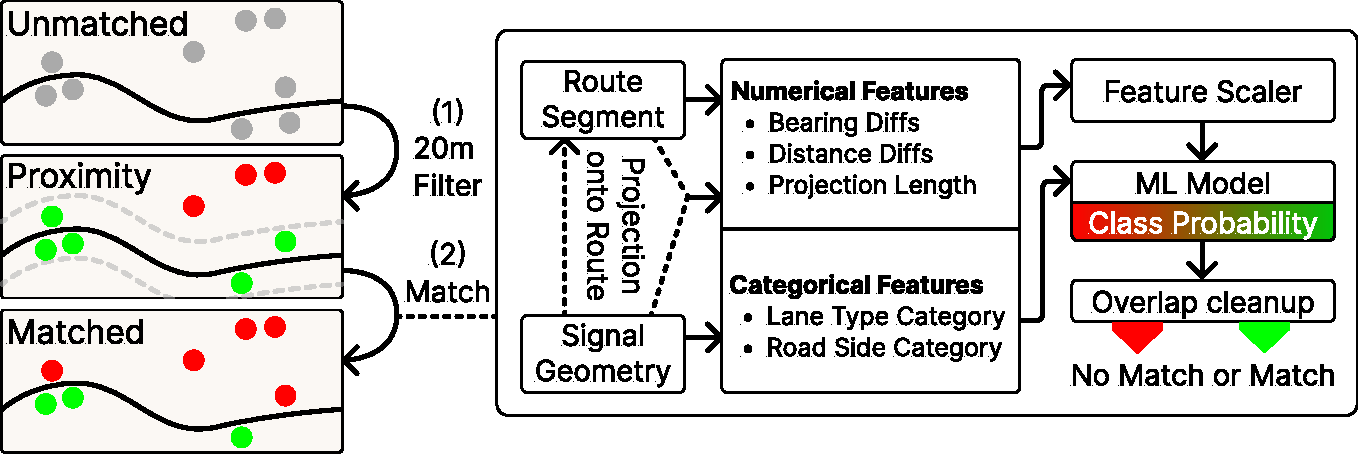
\includegraphics[width=\linewidth]{images/sg-matching-ml-model.pdf}
\caption{Filtering steps for matching with the ML model. Source: \cite{matthes2023geo}}
\label{fig:sg-matching-ml-model}
\end{figure}

The proposed approach (see \Cref{fig:sg-matching-ml-model}) operates as follows: The bearing, length, and overlap filtering steps from the algorithmic approach are removed and replaced with a single "Match" step to incorporate the ML classifier into the filtering process. During this step, the traffic light's geometry is first projected onto the route. The result of this step is one sample incorporating the traffic light geometry and the projected traffic light geometry onto the route. It is important to note that each sample considers one traffic light, not a complete intersection. Based on the sample, numerical and categorical features that represent the geometrical relationship between the route and the traffic light geometry are calculated.

The numerical features are subjected to a feature scaler to prepare them for model inference. The categorical features are calculated or extracted from the traffic light metadata. Both numerical features and categorical features are input into the ML model. As a result, the ML model produces a class probability for "match" or "no match." The class probability is utilized in an additional overlap cleanup step (similar to the algorithmic approach's overlap filter) to obtain the final matching traffic lights along the route.

\paragraph{Feature and Model Grid Search:} To select a suitable ML model architecture and feature processing pipeline, gathered experiences from hyperparameter tuning were utilized to systematically and rigorously identify promising configurations. Out of the tested traditional model architectures including k-Nearest-Neighbors (k-NN), Decision Tree, Random Forest, Multilayer Perceptron (MLP), AdaBoost, Gaussian Naive Bayes, Quadratic Discriminant Analysis (QDA), and Support Vector Machine (SVM), the MLP model overall performed the best and was thus selected as the final classifier, after testing other promising models with different feature constellations. 

To ensure comparability during the model testing process, each model feature pipeline was trained and tested using the stratified variant of the k-fold cross-validation\footnote{\url{https://scikit-learn.org/1.3/modules/generated/sklearn.model_selection.StratifiedKFold.html}}. As there are many more non-matching traffic lights along routes in the ground truth than matching traffic lights, this variant ensures that a similar balance is present in each generated training/testing split of the ground truth dataset. Some features were discarded by looking at the models' scores and the mutual information of each feature, as they provided no additional information. The final feature set is as follows:

\begin{itemize}
    \item The lane type of the traffic light. This property is extracted from the traffic light's metadata and one-hot-encoded.
    \item The roadside of the traffic light. To calculate this property, it is determined on which side of the route the first coordinate of the traffic light geometry is located.
    \item The maximum and minimum bearing diffs between the traffic light geometry segments and their projections onto the route ($\bar{\Delta}_{bear_i}$).
    \item The change in route bearing from the first to the last route segment. 
    \item The first, last, and shortest distance between traffic light geometry coordinates and their projections onto the route.
    \item The length of the traffic light geometry's projection onto the route.
\end{itemize}

A feature scaling algorithm is employed to optimize the ML model's learning and inference process. Here, it is usually a good option to choose a Yeo-Johnson power transformation \cite{yeo_new_2000}, which includes standardization and tries to symmetrize the observed data into a normal distribution. Together with the scaled numerical features, the one-hot-encoded categorical features are input into the model as, in sum, 16 features. Together with the model, the parameters of the Yeo-Johnson power transformation are only fit to the dataset's training proportion.

\begin{figure}[b]
\centering
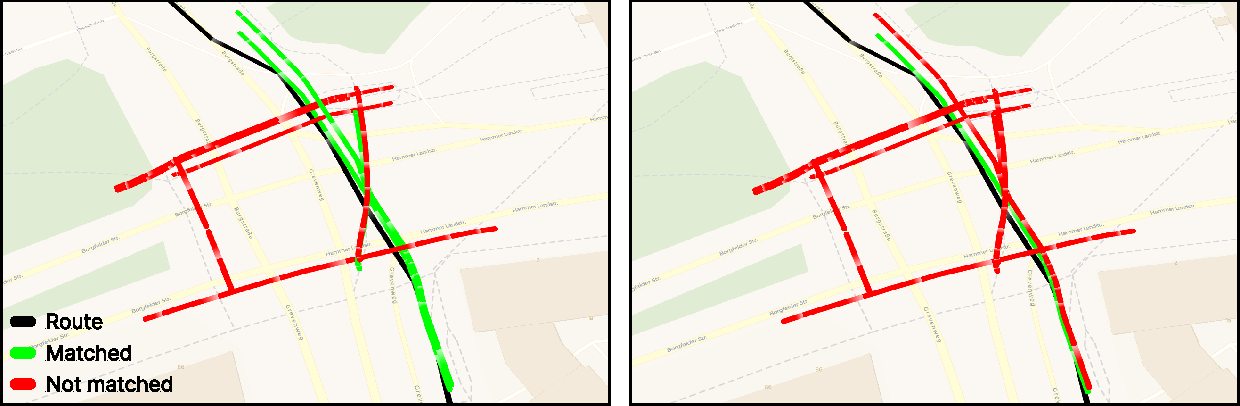
\includegraphics[width=\linewidth]{images/sg-selection-overlap-cleanup.pdf}
\caption{Model selection without (left) and with (right) overlap cleanup. Source: \cite{matthes2023geo}, [\hyperref[attribution]{Attribution}]}
\label{fig:sg-selection-overlap-cleanup}
\end{figure}

\paragraph{Overlap Cleanup:} As in the algorithmic approach, there may be some cases where multiple overlapping traffic lights are selected. These duplicate selections may happen when multiple traffic light geometries are closely aligned to the route and must be cleaned up, as the app should only focus on the traffic light most likely used. 

As shown in \Cref{fig:sg-selection-overlap-cleanup}, the utilized traffic light is most likely the longest of the three selected geometries. This traffic light arguably has the best alignment with the route geometry. How much the model thinks a traffic light matches the route can be measured by the output probability (neuron activation) for the two classes "match" and "no match." This feature is used to force the model to decide between overlapping traffic lights. If a sufficient overlap between two traffic light geometries is detected, the traffic light with the higher probability for "match" is selected. The result of this process is highlighted in \Cref{fig:sg-selection-overlap-cleanup}.

\subsection{Integration of Unconnected Intersections}

Not all intersections have traffic lights connected to Hamburg's data broker. However, this represents a problem for matching traffic lights along a route. If an unconnected intersection lies between the user and the next connected intersection, the user may get a speed advisory for the wrong intersection. Although the traffic light is later visualized on the in-app map, this may confuse the user. Thus, it is crucial also to identify the unconnected intersections along the bike path. These unconnected intersections are later visualized with a unique traffic light symbol in the user interface.

To find out which intersections are not connected to the system (but still signalized), the Lichtsignalanlagen Hamburg\footnote{\url{https://metaver.de/trefferanzeige?docuuid=C498DEED-985C-11D5-889E-000102B6A10E}} dataset is utilized. This dataset is updated periodically every four months and contains single coordinates of each signalized intersection in Hamburg. Thus, the dataset does not resolve individual traffic light geometries but the center locations of the intersection node. 

To identify which intersections are connected, it is determined which intersections have traffic light geometries within an empirically defined threshold of 50 meters. These intersection nodes from the Lichtsignalanlagen Hamburg dataset are marked as "connected." All other nodes are marked as "unconnected." In case of a traffic light unassigned to any intersection node, it is assumed that it is missing in the Lichtsignalanlagen Hamburg dataset, and a new intersection node is created. 

Finally, a list of intersection nodes is matched to the route by a distance threshold of 50 meters. To avoid displaying a speed advisory for a wrong intersection, the app handles each unconnected intersection like a traffic light that does not send any data. Once an unconnected intersection is passed before another (connected) traffic light, the speed advisory is enabled again. This step completes the traffic light matching pipeline.

\begin{Summary}[Summary of Methods]
Route-based traffic light matching is proposed as a novel solution to the problem of identifying traffic lights for GLOSA. The proposed method is designed to be practical for all smartphone mounting spots and invulnerable to inaccurate GNSS. Furthermore, all upcoming traffic lights are known anytime during the ride. However, a significant challenge is precisely estimating which traffic light sequence will most likely be utilized by a cyclist. The approach must employ human-like spatial reasoning to distinguish non-matching from matching traffic lights.

To develop and test mathematical models to resemble human spatial reasoning, human matchings of traffic lights along randomized routes are collected through a web tool. The resulting ground truth dataset is utilized to calculate an overall matching quality through the F1 score.

Multiple methods were tested preliminarily but not investigated further. Nonetheless, the learnings from these methods were ultimately incorporated into an algorithmic filtering pipeline. This pipeline employs geometrical filters that calculate each traffic light's distance, bearing, and projection length to determine whether it would suit the route. Finally, overlapping traffic lights are compared to each other to decide which one matches the route better. As a result, a sequence of traffic lights is returned, which are predicted to match a given input route.

To further improve the developed filtering pipeline, it was determined that the geometric features, such as bearing or projection length, could be weighted more dynamically by an ML model. The final MLP model developed by Daniel Jeschor \cite{jeschor_2022} utilizes 16 features calculated from the traffic light's geometry and its projection onto the route to determine if this traffic light matches the route. In case of overlaps, the traffic light predicted to match the route most likely is chosen.

Finally, to avoid speed advisories being given for a traffic light that comes after an unconnected but signalized intersection, the Lichtsignalanlagen Hamburg dataset is utilized. 
\end{Summary}

\section{Results}

The evaluation of the traffic light matching process is divided into several parts. We begin with the data analysis of traffic light geometries and then proceed to examine the Ground Truth. We assess whether the Ground Truth is representative enough to make qualified statements about the accuracy of the developed procedures. Using these considerations, we then evaluate the benchmark performance of both approaches. Additionally, we investigate how effectively both methods select the correct traffic lights, even in the presence of routing errors. The matching time and practicality of the final model are examined through a short performance analysis on a TU-Dresden deployment. Finally, we validate our benchmark results through a test in Hamburg.

\subsection{Study of Traffic Light Geometries in Hamburg}

Initiating the evaluation, we first take a closer look at traffic light geometries. The concept emphasizes that meta-information about the modes of transportation served by a traffic light is a crucial decision criterion. The developed procedure should consistently choose a dedicated bicycle traffic light when feasible based on the intersection topology. Thus, it is vital to understand the spatial distribution and shape patterns of bicycle traffic light geometries.

As of December 8, 2023, 85.6\% of the 791 available intersection nodes in the system have at least one dedicated bicycle traffic light. At 24.5\% of intersections, at least one traffic light is shared between cyclists and motor vehicles, and 6.7\% have lights designated for mixed traffic involving cyclists, motor vehicles, and buses. 3\% of intersections feature lights shared between pedestrians and cyclists.

\begin{figure}[t]
\centering
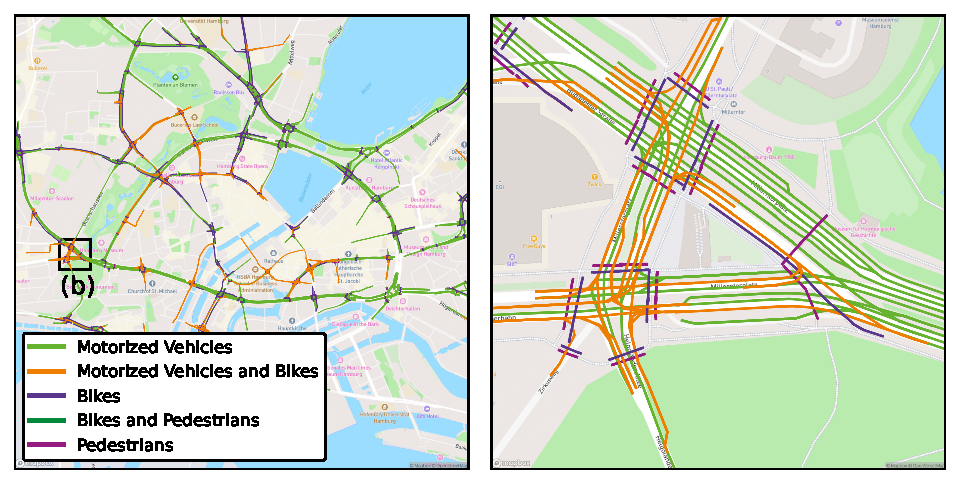
\includegraphics[width=\linewidth]{images/lanes-map.pdf}
\caption{Types of transport modes served by traffic lights in Hamburg (extracted from metadata). [\hyperref[attribution]{Attribution}]}
\label{fig:lanes-map}
\end{figure}

As shown in \Cref{fig:lanes-map}, the percentage overlap occurs because there are often multiple parallel traffic lights per intersection and direction, providing theoretical choices for cyclists, but only one ultimately proves to be the optimal option. Examining individual ingress lanes and potential turns from these lanes reveals that cyclists frequently have numerous options to turn in the same direction. Of 4349 marked ingress lanes for cyclists, 653 (15\%) are associated with multiple traffic light geometries. For instance, at intersection 177\footnote{\url{https://www.google.com/maps/place/53\%C2\%B034'10.6\%22N+10\%C2\%B003'22.1\%22E}}, cyclists can turn right into four lanes, left into four lanes, and proceed straight from a single ingress lane.

While multiple connections typically operate simultaneously, and an incorrect choice does not necessarily lead to a wrong speed recommendation, it is essential to consider that different turning directions may be served by separately operating traffic light controllers.

In cases where the nearest traffic light geometries overlap, a proximity-based selection may be ambiguous, potentially leading to a displayed speed advisory for the wrong turning direction. Additionally, several parallel ingress lanes can often be independently controlled, such as a bicycle traffic light preceding a vehicle traffic light also tagged for cyclists. Although these lanes do not physically overlap, they are usually only a few meters apart.

\begin{figure}[t]
\centering
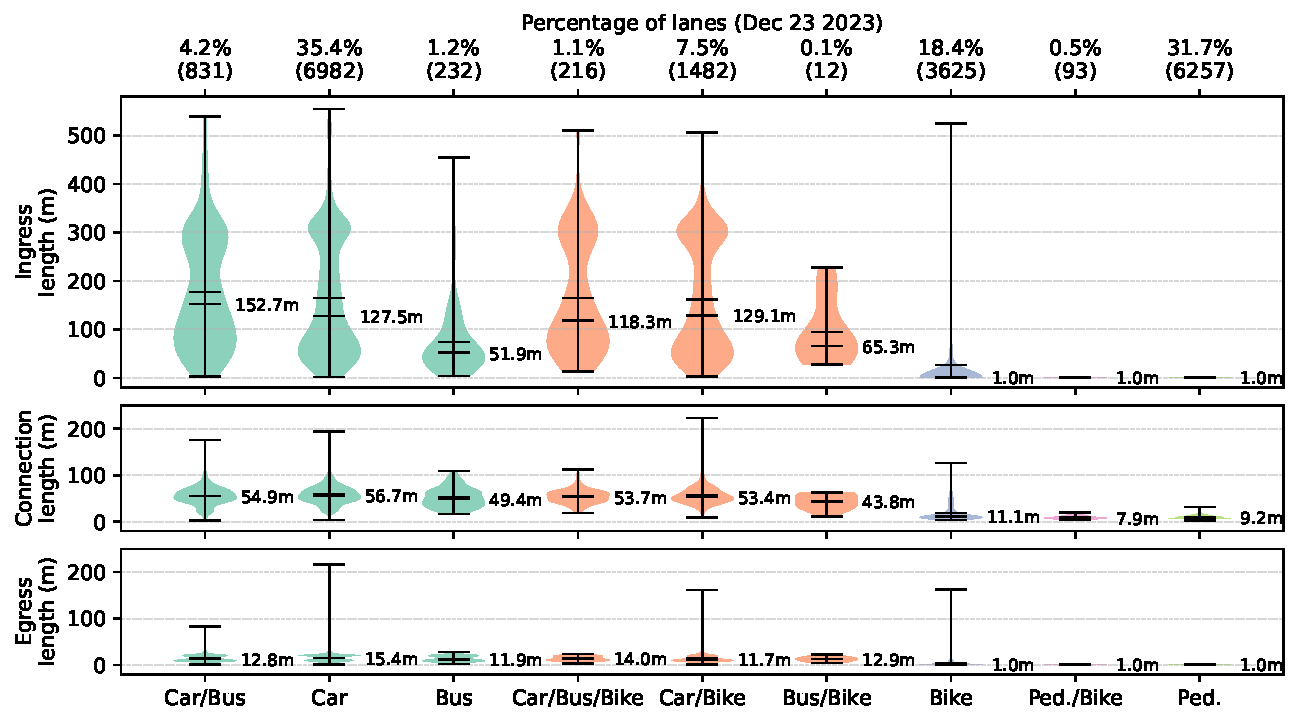
\includegraphics[width=\linewidth]{images/lanes-lengths.pdf}
\caption{Lane lengths of traffic lights in Hamburg as measured through the Vincenty distance.}
\label{fig:ingress-lane-lengths}
\end{figure}

Another challenge is the issue of ingress lane length. As depicted in \Cref{fig:ingress-lane-lengths}, it is generally reasonable to assume a non-too-short ingress lane length for cars and use it for matching. However, contrary to Stahlmann et al.'s report (2018) \cite{stahlmann_exploring_2018}, link lengths of 590 to 910 meters cannot be observed. Even when the ingress, connection, and egress lane geometries are combined, the total length is well below 300 meters. A timely speed advisory activation for these traffic lights will require predicting in some way that the user is currently moving toward them.

For cyclists, the situation is much more problematic. As initially described, the issue for cyclists is that many traffic lights can be approached from multiple directions. The result is visible in \Cref{fig:ingress-lane-lengths}, with ingress lane lengths, if all (including shared) bicycle lanes marked in the diagram are considered together, having a median length of 1 meter. In many cases, ingress lanes would need to be artificially extended in multiple directions, or at least multiple longer ingress lanes would need to be provided. This would require a restructuring of all intersection topologies.

Even then, the problem is not entirely resolved, as the ingress lanes of multiple traffic lights would overlap, leading to an unclear mapping of which traffic light the user is approaching. These results confirm that any location-based matching method without knowledge of the actual turn taken at the upcoming intersection is severely limited for cyclists. The ambiguity in approaching the traffic light would be too significant in many cases to make a precise selection, even assuming perfect GNSS accuracy.

\subsection{Analysis of Ground Truth}

The development of the route-based matching method involved creating several ground truths, which we will now examine in more detail.

\begin{figure}[t]
\centering 
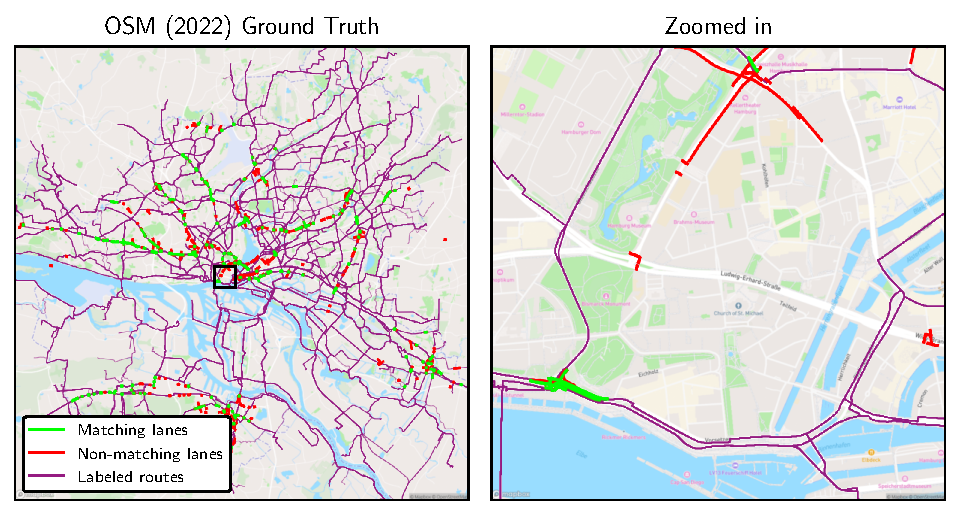
\includegraphics[width=\linewidth]{images/matching-ground-truth-osm-old.pdf}
\caption{OpenStreetMap 2022 ground truth for model training and evaluation. [\hyperref[attribution]{Attribution}]}
\label{fig:matching-ground-truth-osm-old}
\end{figure}

The first ground truth was established in 2022 and consists of 148 randomly generated bicycle routes through Hamburg using OSM and the GraphHopper \texttt{bike2} profile. This ground truth is illustrated in \Cref{fig:matching-ground-truth-osm-old}. The ground truth was constructed using a dataset of traffic light geometries containing 2414 individual connections available in 2022. A total of 1043 traffic lights were manually assigned to the 148 routes. On average, each route encompasses seven traffic lights.

In \Cref{fig:matching-ground-truth-osm-old}, the manually assigned traffic lights (in blue) are marked in green, while traffic lights that were never assigned are marked in red. It is noticeable that some traffic lights were never selected, mainly due to two reasons: some intersections were not traversed by any generated route, and at traversed intersections, there are often traffic lights that never constitute a meaningful match. In extreme cases, there are intersections where no traffic light matches the route, perhaps because it is irrelevant to the bike path alongside the road.

Along the 148 routes, 6440 connections were considered at least once while labeling the ground truth, with 5397 (83.8\%) marked as "no match." This pertains to all traffic lights within the 20m radius, always drawn around the route. Therefore, the matching method must label significantly more connections as "no match" in the matching process than as "match."

While only 549 unique connections are identified at least once as a "match," an additional 1231 unique connections are never identified as a "match" despite being considered. Consequently, the 2022 OSM dataset covers 73.7\% (1780) of all 2414 traffic lights, although it does not necessarily account for all possible entry directions of the intersections.

\begin{figure}[t]
\centering 
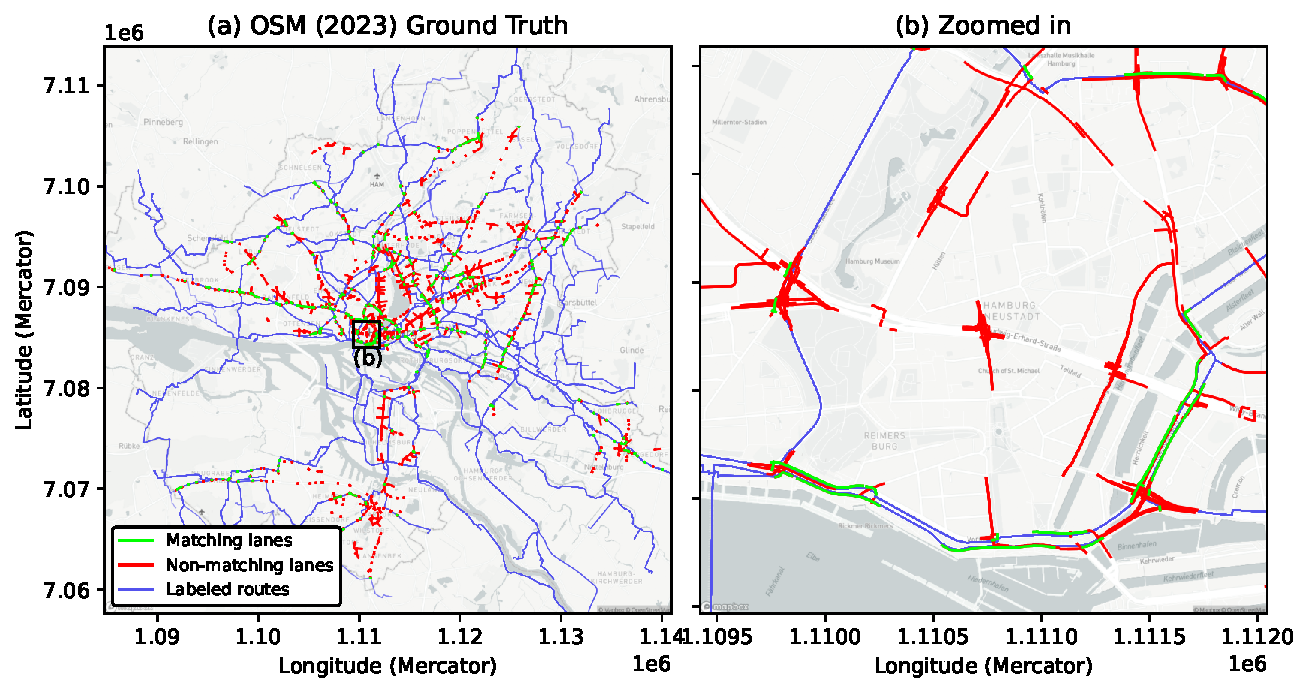
\includegraphics[width=\linewidth]{images/matching-ground-truth-osm.pdf}
\caption{Additional OpenStreetMap 2023 ground truth for model training and evaluation. [\hyperref[attribution]{Attribution}]}
\label{fig:matching-ground-truth-osm}
\end{figure}

A limitation of the first ground truth is its inclusion of only 2414 connections, representing 44\% of the 5486 connections available as of December 13, 2023.

To address this limitation, a second ground truth was created in 2023 to validate the models and results using the 2022 ground truth. This new ground truth contains 5168 connections, accounting for 94.2\% of the available connections, as depicted in \Cref{fig:matching-ground-truth-osm}. The 2023 ground truth consists of 52 routes generated using the same schema and 758 connections marked as "match." This equates to approximately 15 connections per route, consistent with the increased coverage.

Notably, adding new routes to the ground truth does not necessarily result in adding new connections. Since multiple routes can traverse an intersection in a similar manner, each newly added route tends to contribute fewer new traffic lights to the dataset.

An implication of this is that there is a limit to the number of routes that can be meaningfully added to the dataset. With each new route, there is an increased risk of introducing duplicate examples. Excessive duplicates should be avoided to minimize dataset bias. Specifically, when training an ML classifier, an abundance of duplicates can lead to overfitting and reduced generalization capability.

\begin{figure}[t]
\centering 
\begin{tabular}{cc}
\footnotesize{(a) Redundancy in OSM Ground Truth (2022)} & \footnotesize{(b) Redundancy in OSM Ground Truth (2023)} \\
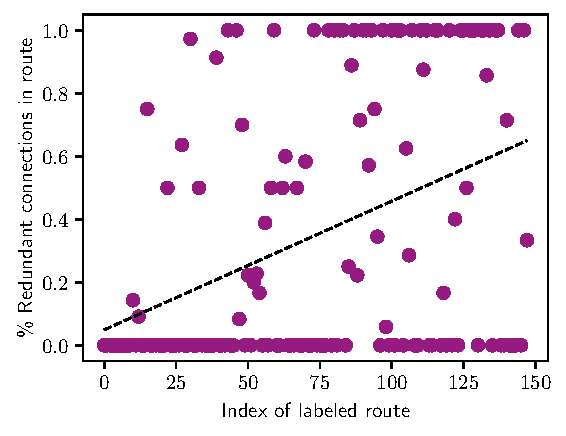
\includegraphics[width=0.45\linewidth]{images/matching-ground-truth-progression-osm-old.pdf} & 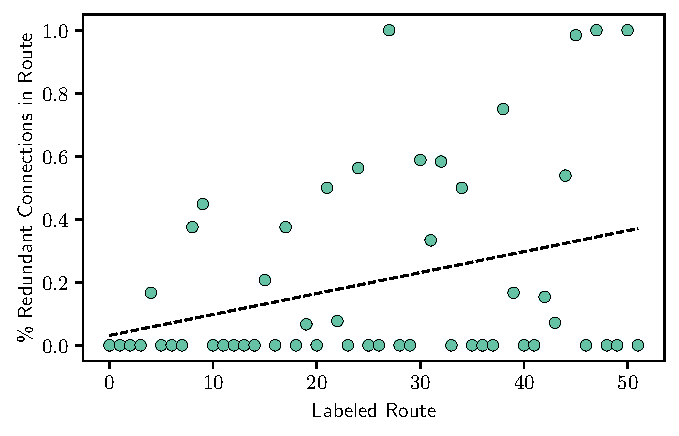
\includegraphics[width=0.45\linewidth]{images/matching-ground-truth-progression-osm.pdf} \\
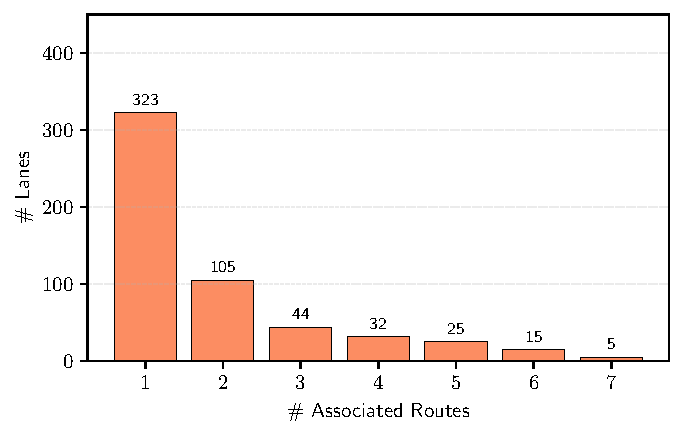
\includegraphics[width=0.45\linewidth]{images/matching-ground-truth-lsas-per-route-osm-old.pdf} & 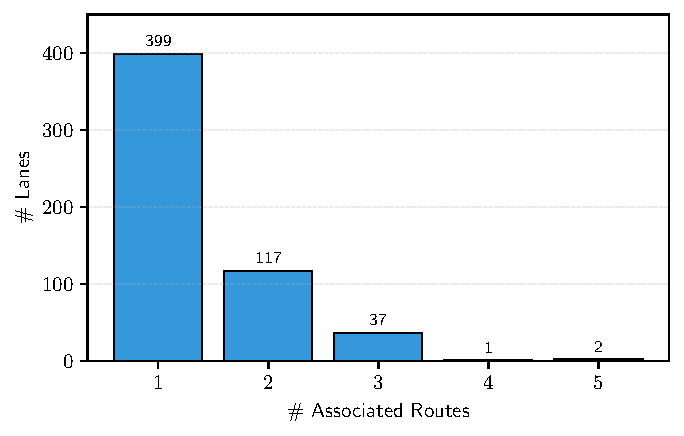
\includegraphics[width=0.45\linewidth]{images/matching-ground-truth-lsas-per-route-osm.pdf} \\
\end{tabular}
\caption{Redundancy of each ground truth as indicated by new constellations and multiple assignments to routes.}
\label{fig:ground-truth-routes-per-lanes-osm}
\end{figure}

The relationship is more precisely illustrated in \Cref{fig:ground-truth-routes-per-lanes-osm}. For each new route, it was determined how many "match"-marked connections already existed in the dataset. Since more routes were labeled in the 2022 OSM dataset than in the 2023 OSM dataset, the redundancy of new routes tends to be higher.

We can estimate the likelihood of encountering previously seen connections in added routes through the trend of added redundant connections. Assuming a linear relationship, as depicted by the dashed line in \Cref{fig:ground-truth-routes-per-lanes-osm}, the probability is 65\% for the 2022 OSM dataset and 38\% for the 2023 OSM dataset.

In conclusion, we cannot add unlimited routes to the ground truth without encountering redundancy issues. The decision on where to terminate the creation of new routes is somewhat arbitrary. In creating the 2023 OSM dataset, this decision was made earlier than in the 2022 OSM dataset.

This creation process results in most lanes (connections) being assigned to only one route. As shown in \Cref{fig:ground-truth-routes-per-lanes-osm}, this applies to 323 routes in the 2022 OSM dataset and 399 routes in the 2023 OSM dataset. In the 2022 OSM dataset, isolated lanes are assigned to up to seven routes.

Overall, the distribution indicates that there may be significantly more duplicates in the 2022 OSM dataset compared to the 2023 OSM dataset. Whether these duplicates are excessive cannot be accurately assessed without testing the model's generalization capability on unseen data, which we will address in detail in the next section.

\subsection{Model Evaluation}

Two models were designed: the algorithmic model and the ML model. Each model was trained and evaluated on the ground truths presented in the previous section. First is the algorithmic model. The same version of the algorithmic model was trained once on the 2022 OSM dataset and once on the 2023 OSM dataset. This separate training resulted in two distinct models validated on the other dataset.

\begin{table}[t]
\caption{Tuned hyperparameters for the algorithmic matching model.}
\resizebox{\linewidth}{!}{\begin{tabular}{@{}llllllllll@{}}
\toprule
\textbf{Ground Truth} & $t_{dist}$ & $t_{bear}$ & $t_{bear\_sum}$ & $t_{inv}$ & $t_{len}$ & $t_{len\_sum}$ & $t_{road\_side}$ &  $t_{perfect\_m.}$ & $t_{overlap}$ \\
  \midrule
  OSM (2022) & 20m & 33° & 79\% & False & 0.99 & 93\% & 59m & 50m & 43\% \\
  OSM (2023) & 19m & 50° & 78\% & False & 0.96 & 77\% & 95m & 46m & 5\% \\
\bottomrule
\end{tabular}}
\label{tab:hyperparameter-tuning-results}
\end{table}

The specific model configurations are detailed in \Cref{tab:hyperparameter-tuning-results}. The hyperparameter tuning process selected similar values for the initial thresholds along the filter pipeline. Ignoring the parameters of the overlap matchers initially, notable differences are observed only in the chosen bearing threshold $t_{bear}$ and the length filter. While the 2023 model is less strict in filtering steeply angled lane geometries, the length filter is configured more rigorously. This is not surprising, as the bearing and length filters pertain to similar properties between the route and the lane. The overlap matcher, which comes last in the filter pipeline, exhibits more pronounced differences between the two model variants. 

\Cref{fig:hyperparameter-contourplot} provides more detailed insights into interpreting the hyperparameter tuning. The figure shows the direction in which the parameter configuration was estimated to improve the maximum F1 score. As a foundation, this plot was generated using the training history of the 2023 model.

Several interesting conclusions can be drawn from the figure regarding the training and the general interpretation of a "good" match between a route and a traffic light geometry. First, a clear trend is observed with Threshold 5, which decides whether inversely oriented traffic light geometries should be chosen as a match. The tendency is clearly towards "no," aligning with Rule 6 in the dataset creation, stating that traffic light geometries should never be chosen against the direction of travel. 

\begin{figure}[t]
\centering 
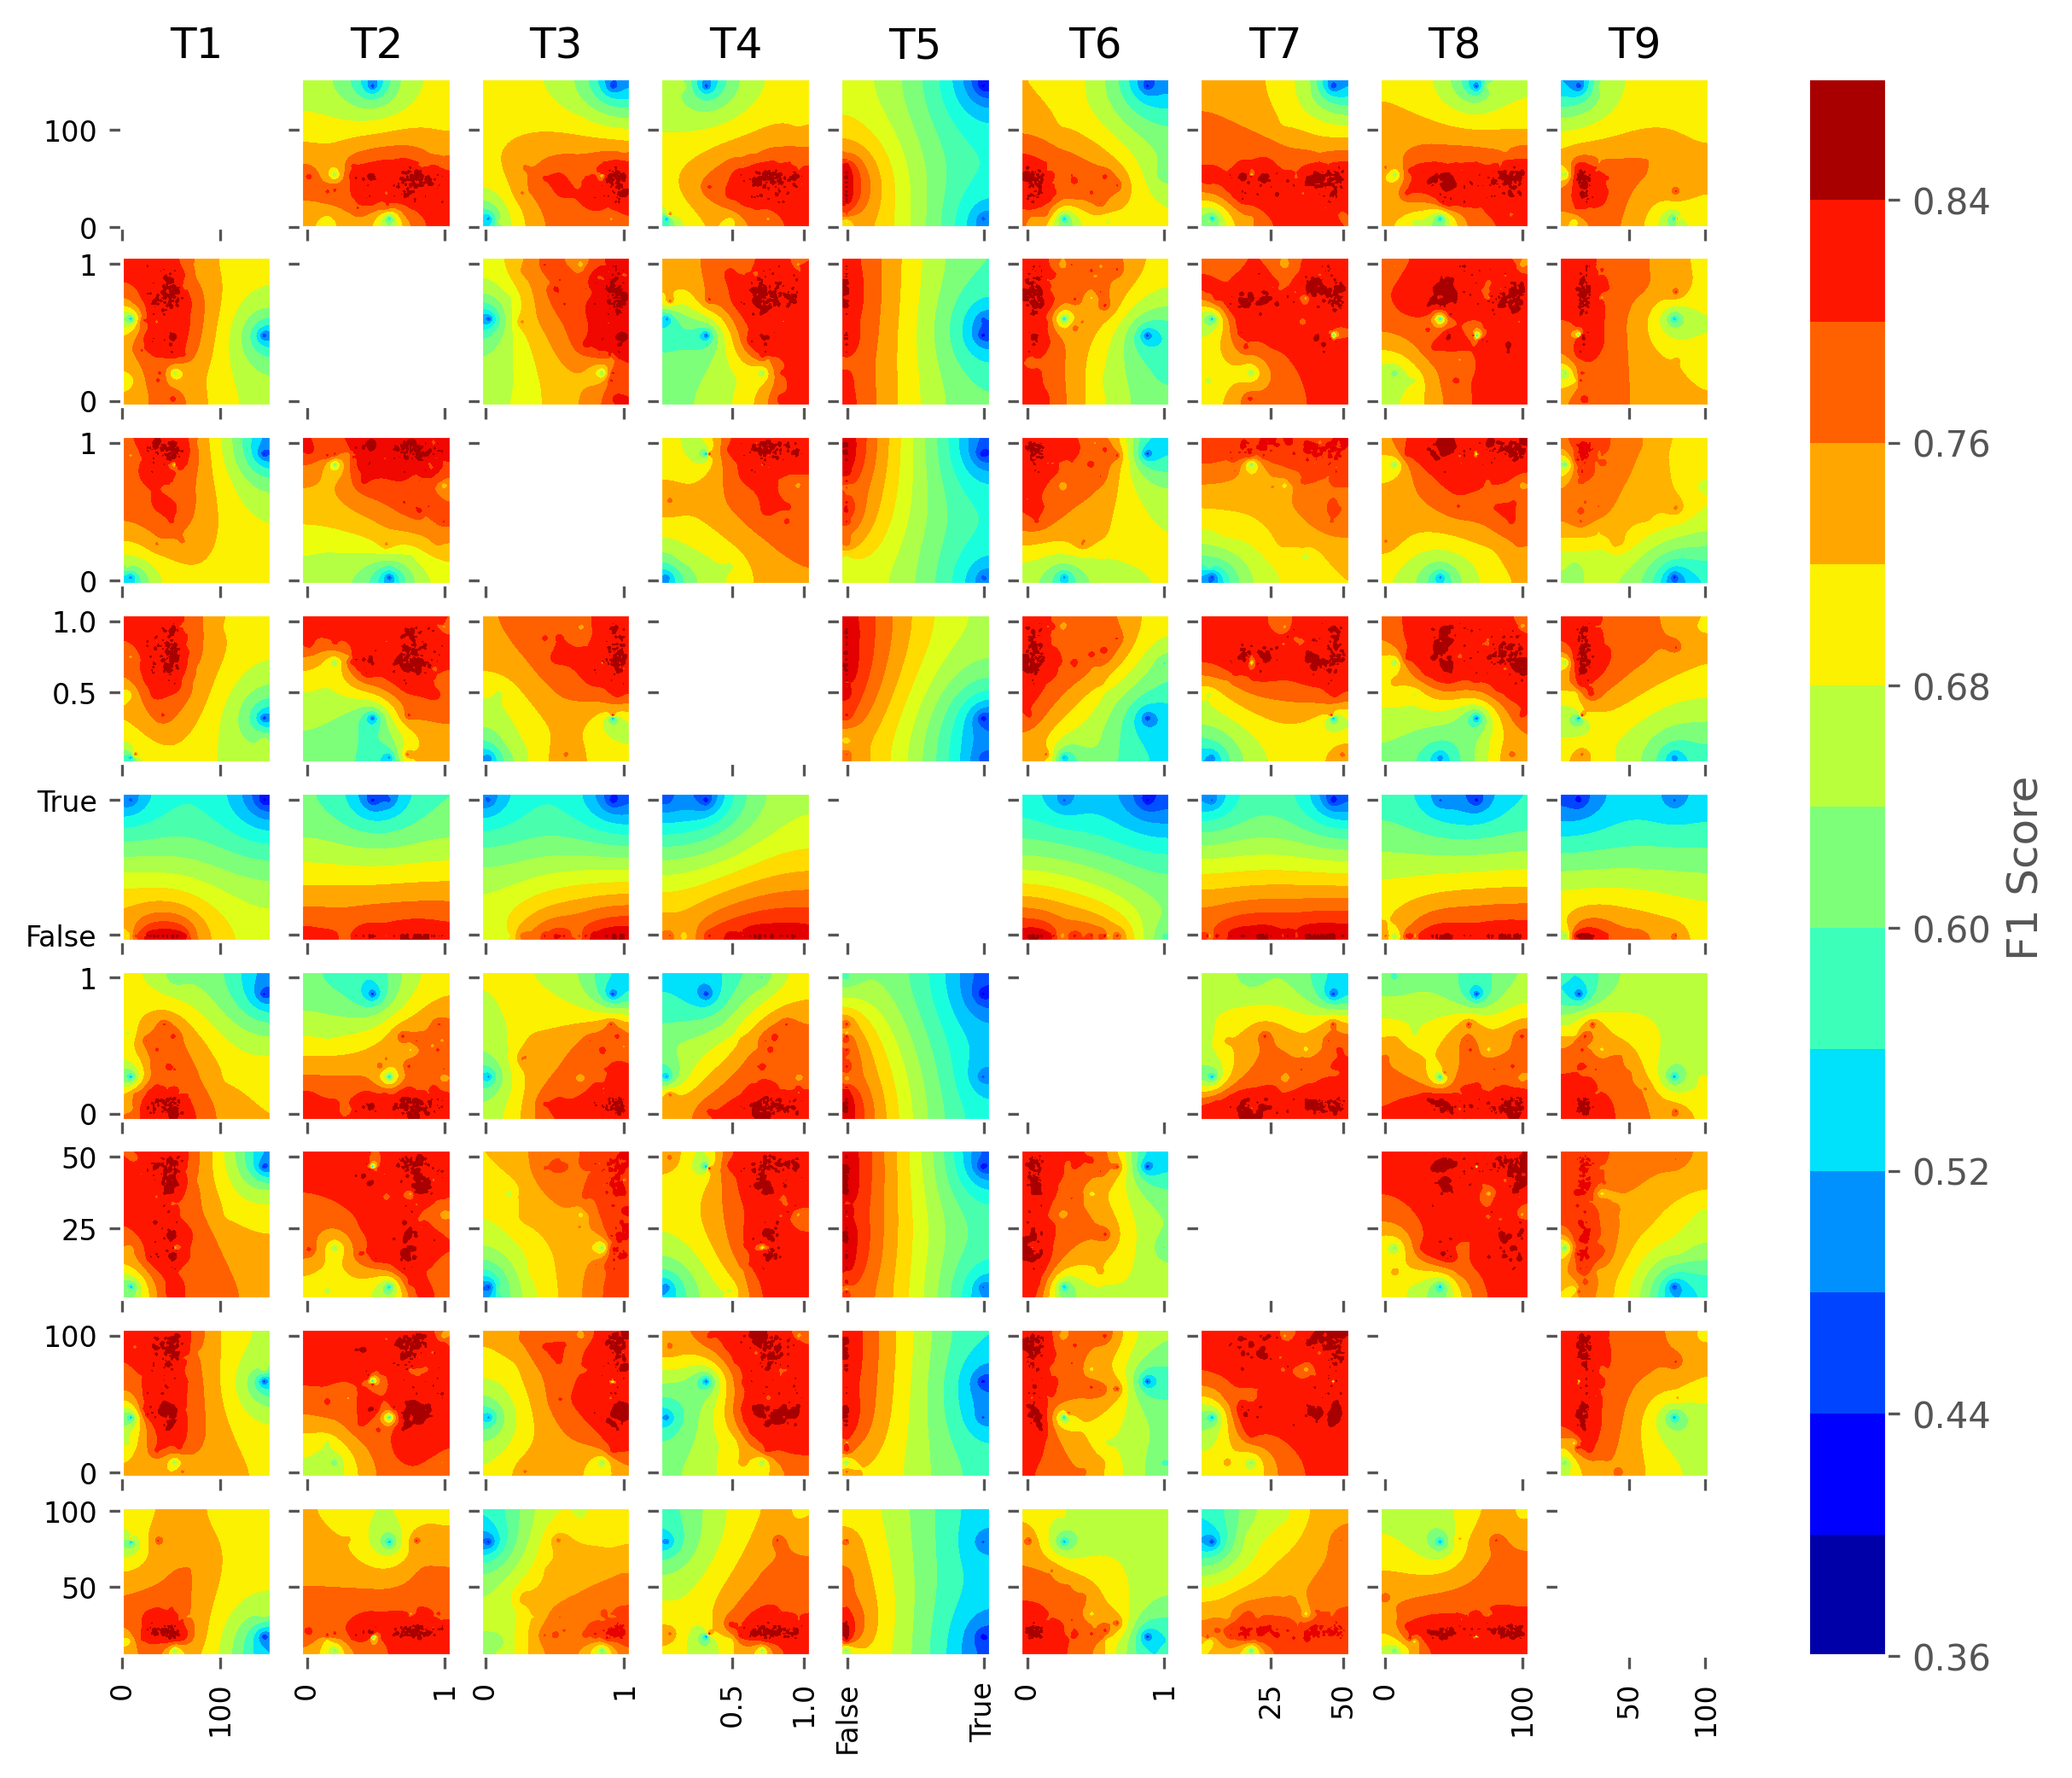
\includegraphics[width=\linewidth]{images/matching-hpt-contour-topological-osm-updated.png}
\caption{Contour plot of the hyperparameter tuner's threshold search space indicating its gradient measurements for F1 score optimization.}
\label{fig:hyperparameter-contourplot}
\end{figure}

The hyperparameter model successfully reconstructed this relationship. Clear gradients are also noticeable at other thresholds. The loss gradients for the overlap thresholds T7 to T9 appear diffuse, aligning with the variability observed in these parameters in the final models. Overall, the hyperparameter tuning appears to have captured essential relationships effectively. At least, no better model could be manually found.

The ML model was trained on the 2022 OSM dataset and is evaluated on both OSM ground truths. The training and evaluation of the ML model need to be conducted with more care to address overfitting issues effectively via regularization. Caution is indicated here as the ground truth analysis revealed increased redundancy, especially in the 2022 OSM dataset. Since this is also the dataset on which the ML model is trained, 3092 out of 6440 redundant examples were identified and removed based on matching feature vectors before training. The model training was conducted using Stratified K-Fold Cross-Validation over 342 epochs.

\begin{figure}[!t]
\centering 
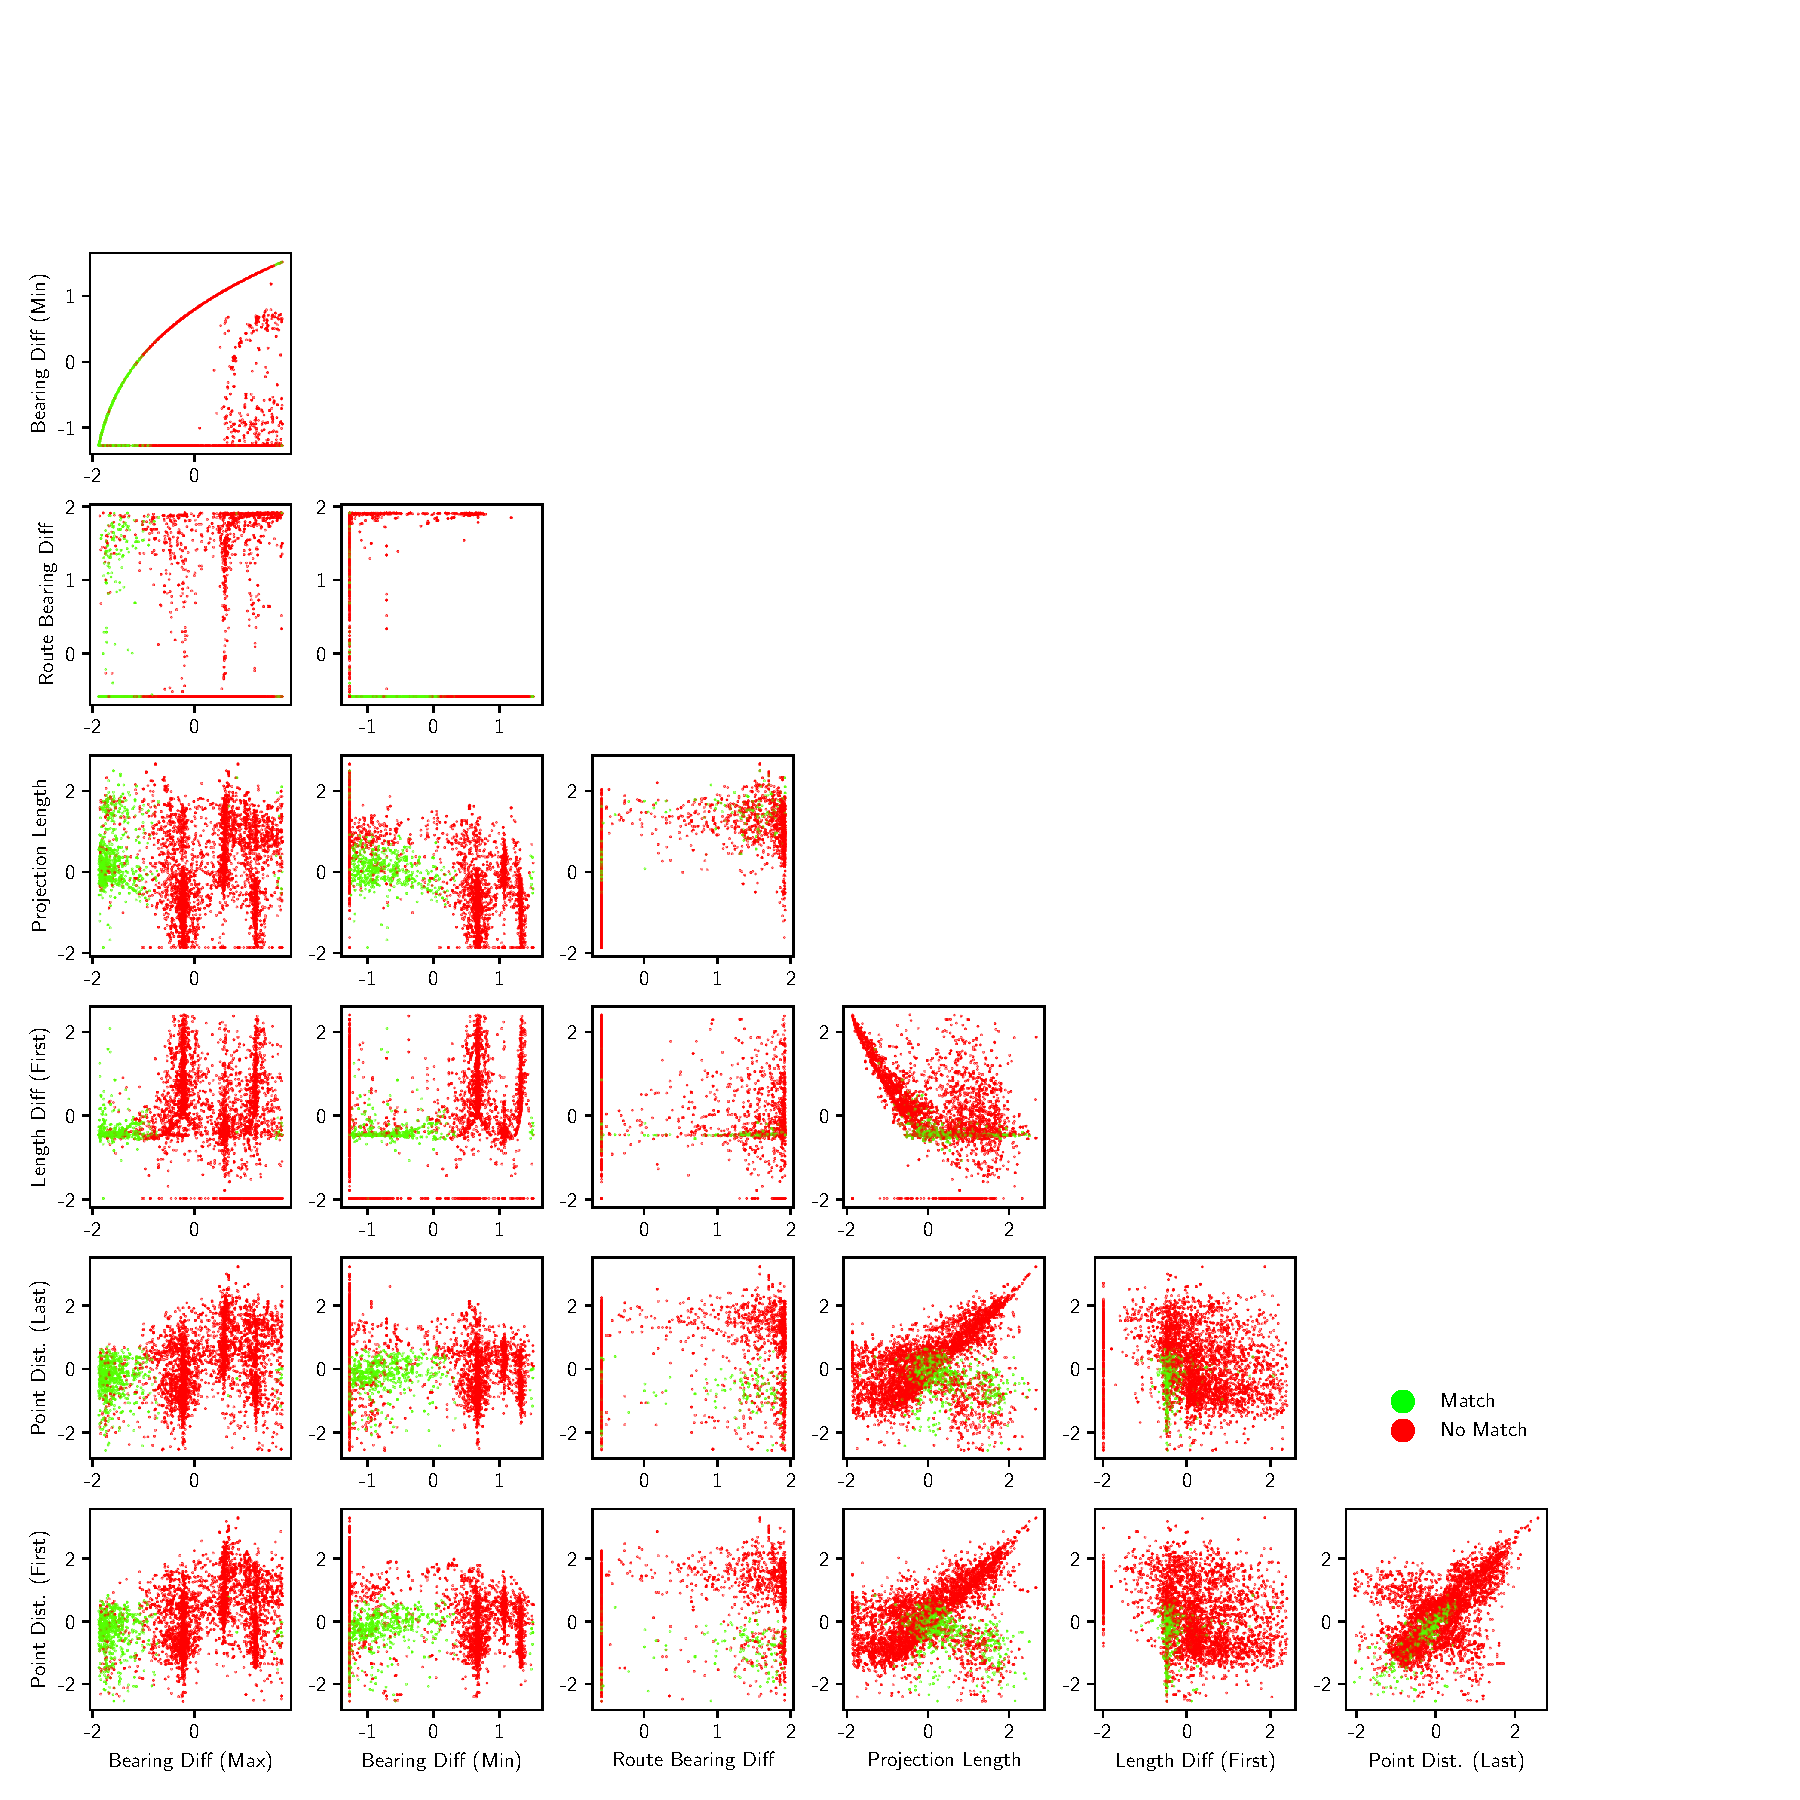
\includegraphics[width=\linewidth,bb=0 0 760 760]{images/decision-boundaries.pdf}
\caption{Decision boundaries of the ML model's Yeo-Johnson-transformed non-categorical features.}
\label{fig:ml-model-decision-boundaries}
\end{figure}

A look at the decision boundaries of the trained ML model allows us to gain a more precise understanding of its workwise. The gradual decision boundaries of the non-categorical features are shown in \Cref{fig:ml-model-decision-boundaries}. This visualization was created by inferring random routes on the model and recording the calculated features along with the predicted class. 

Since the input values have already been transformed into the feature space through the Yeo-Johnson transformation, the depicted relationships may not be evenly distributed across the input data. However, it is visible, especially in the bearing features (max and min), that input values mapped to 0, which should lie around 180° opposite to the route, serve as exclusion criteria for non-matching lanes.

When the lane and the route are very close to each other (Point Dists), this is another strong indicator of a match. However, the observation that even near the zero line of Point Distances, where lanes presumably lie very close above the route, there are still many non-matching lanes is also interesting. Consequently, the distance to the route is likely not a sole decision criterion, even for well-overlapping geometries. The same observation applies to the Length Diff feature.

Having explored the interpretability of the models, we next focus on the achieved scores. These are presented in \Cref{tab:model-scores}.

\begin{table}[ht]
\caption{Model evaluation scores.}
\begin{tabular}{@{}lllllllll@{}}
\toprule
  \textbf{Model} & \textbf{Benchmark} & \textbf{Trained on} & \textbf{TP} & \textbf{FP} & \textbf{FN} & \textbf{Precision} & \textbf{Recall} & \textbf{F1} \\
  \midrule
  Algorithmic & OSM 2022 & OSM 2022 & 920 & 207 & 123 & 82\% & 88\% & 84.8\% \\
  Algorithmic & OSM 2022 & OSM 2023 & 908 & 221 & 135 & 80\% & 87\% & 83.6\% \\
  ML          & OSM 2022 & OSM 2022 & 936 & 57 & 107 & 94\% & 90\% & 91.9\% \\
  \midrule
  Algorithmic & OSM 2023 & OSM 2022 & 615 & 159 & 143 & 79\% & 81\% & 80.3\% \\
  Algorithmic & OSM 2023 & OSM 2023 & 637 & 136 & 121 & 82\% & 84\% & 83.2\% \\
  ML          & OSM 2023 & OSM 2022 & 614 & 52 & 144 & 92\% & 81\% & 86.2\% \\
\bottomrule
\end{tabular}
\label{tab:model-scores}
\end{table}

The algorithmic model trained on the 2022 OSM dataset achieves an F1 score of 84.8\% on the same dataset, while the algorithmic model trained on the 2023 OSM dataset shows an F1 score of 83.6\%. These results suggest the algorithmic approach's robust performance in validating on unknown data, even though a slight loss of accuracy is observed. Both algorithmic models generate relatively many false positives (FP) compared to the number of false negatives (FN), resulting in a low precision score of 82\% and 80\%, respectively.

The ML model trained by Daniel Jeschor \cite{jeschor_2022} on the 2022 OSM data effectively filters out false positives about four times more, yielding a precision score of 94\%. The recall is also slightly higher. Overall, the ML model achieves an F1 score of 91.9\% across the entire dataset, surpassing the comparable algorithmic model by 7.1\%. On the stratified k-fold cross-validation of the duplicate-corrected dataset, the ML model achieves a similar test score of 92\% (94\% training).

After validating the models on the 2023 OSM dataset, those trained on the 2022 OSM dataset performed less well. One possible explanation is that the 2023 OSM dataset contains significantly more connections that, together with the generated routes, represent new, unknown configurations for the model. The loss in the F1 score is mainly reflected in the lower recall, indicating that more traffic lights that belong to the route are being filtered out. Interestingly, even the algorithmic model optimized on the 2023 data performs worse on the 2023 OSM dataset than the model optimized on the larger 2022 OSM dataset. This suggests that a better result could have been achieved if the 2023 OSM dataset had been slightly larger.

Assessing how satisfactory these results are is challenging. Since the presented approach uses user-generated routes rather than real-time GNSS data, comparing it with location-based approaches is challenging. Assuming the user precisely follows the route would be questionable, given the inherent uncertainties in GNSS measurements and the imperfect representation of bike paths in the OSM route. Methodological uncertainties in implementing a location-based approach hinder a meaningful comparison with other methods. The results from Koukoumidis et al. (2011–2012) \cite{koukoumidis_signalguru_2011, koukoumidis_leveraging_2012} cannot be directly compared, as they were calculated based on the number of correctly detected camera images rather than per traffic light. Therefore, an absolute interpretation of the results solely through comparison with other works is not possible, given the substantial differences in the fundamental ideas of the approaches.

Instead, what we can do is carefully examine areas where improvement potential exists and evaluate the approach's performance in real driving scenarios.

\begin{figure}[t]
\centering 
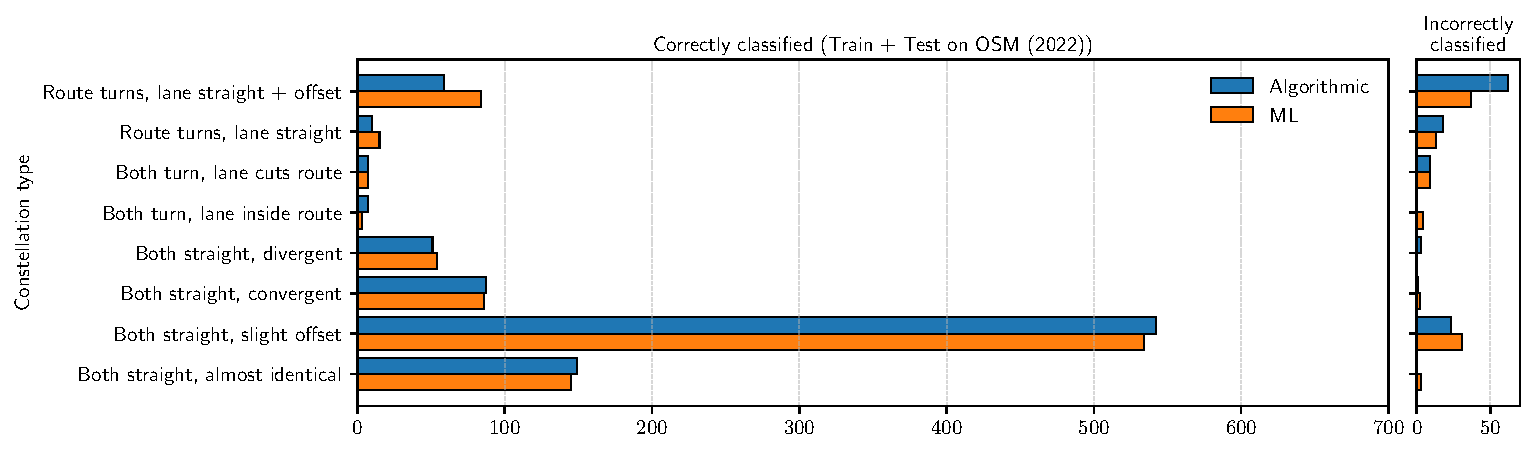
\includegraphics[width=\linewidth]{images/matching-constellations-osm-old.pdf} \\
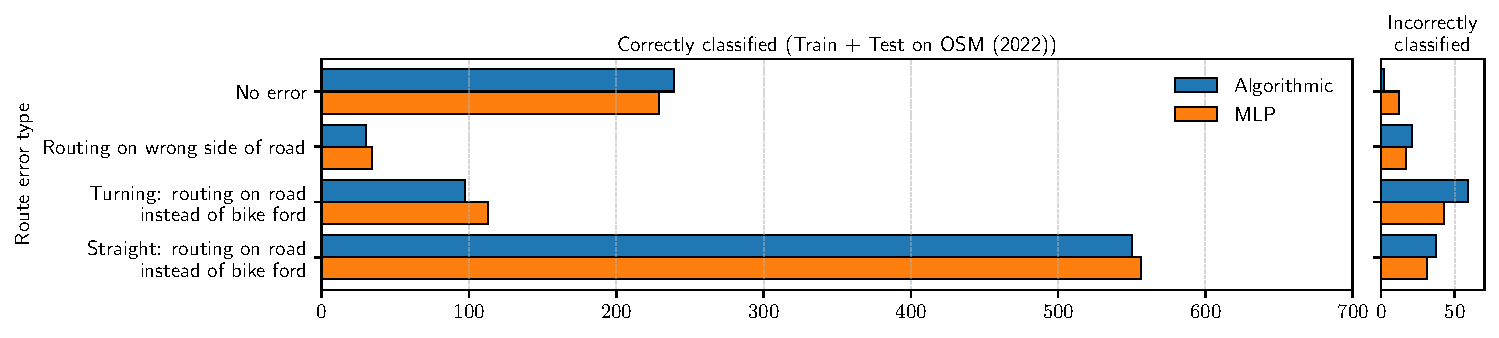
\includegraphics[width=\linewidth]{images/matching-route-errors-osm-old.pdf}
\caption{Recorded types of routing errors and constellation between route and traffic light geometry.}
\label{fig:matching-constellations-osm}
\end{figure}

\Cref{fig:matching-constellations-osm} examines the type of constellation between the route and traffic light geometry, which was specified during the 2022 OSM ground truth creation for each selection. This could provide more detailed insights into the types of constellations where the models can be improved.

By far, the most common constellation is when the route and the lane go straight and are slightly offset from each other. With this constellation, the ML model struggles slightly more than the algorithmic model. Even when both geometries almost exactly overlap and go straight, the ML model achieves a slightly lower score.

On the other hand, the ML model performs significantly better in situations where the route turns, but the corresponding lane goes straight and may also have an offset from the route. This occurs, for example, when the route turns left over the car lanes at an intersection, but a short, straight bicycle traffic light to the right needs to be selected.

These situations occur more frequently than expected and are closely related to the imprecise bicycle routing in OSM.

The analysis of route-lane constellations reveals that only a relatively small number exhibit no routing errors. This assessment involved marking the constellation type in the Route Composer and any occurring routing errors. In the majority of cases, approximately 72\%, the route does not utilize the bicycle lane or bicycle ford at traffic lights but instead follows the center of the road. This occurrence is more than twice as frequent as instances with no routing errors.

In some cases, routing occurs on the wrong side of the street. The ML model demonstrates a higher accuracy of 86\% in detecting routing errors and correctly associating them with the traffic light geometry, surpassing the algorithmic model's 78\% accuracy. When no routing errors are present, the algorithmic model marginally outperforms the ML model with an accuracy of 96.2\% compared to 95.15\%. However, this advantage diminishes significantly due to routing errors associated with OSM.

The ML model proves superior in matching traffic lights compared to the algorithmic model, making it the final model for OSM matching provided to app users. The remaining concerns revolve around evaluating real-world application performance and scalability over longer routes or additional traffic light geometries.

Further insights into user perception of the matching process will be explored in \Cref{ch:app} through user surveys. Meanwhile, our focus here is on quantitative validation in real-world scenarios. Initial considerations involving user tracks for validation were dismissed due to significant GNSS trajectory drift, making it challenging to identify which traffic light was utilized.

An alternative validation method was adopted. On March 21, 2023, four test rides with good prognosis availability were conducted and filmed using a camera. The app calculated routes for these rides, and the final version of the matching algorithm automatically selected traffic lights. Subsequent video analysis confirmed the correct selection of 51 out of 56 passed traffic lights, resulting in an accuracy of 91.07\%. These measured results align with the ground truths, validating the effectiveness of the matching algorithm.

\begin{figure}[t]
\centering 
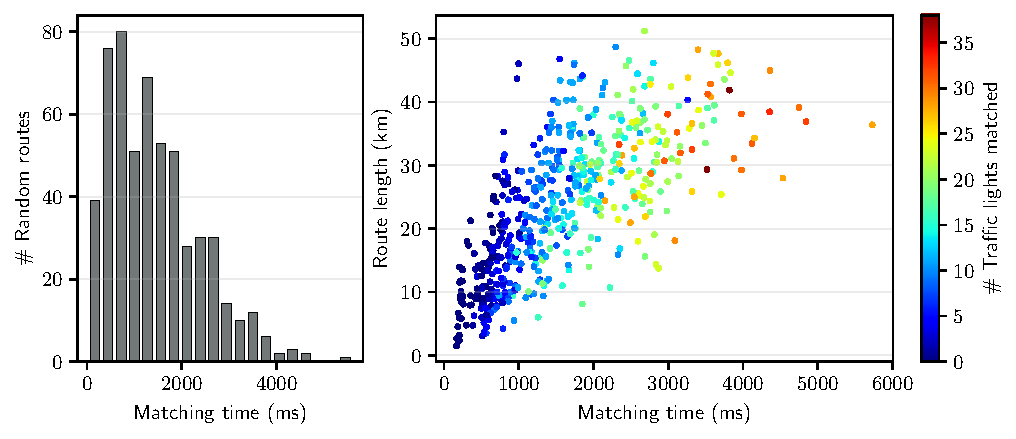
\includegraphics[width=\linewidth]{images/matching-performance-556-routes.pdf}
\caption{Relation between number of traffic lights, route length, and matching time measured on the Beta deployment.}
\label{fig:matching-performance}
\end{figure}

Finally, we examine the response time of the final service using the ML matching method. This metric is crucial as users do not want to wait indefinitely for route calculation and matching. Even in the case of automatic route recalculation, the functionality of speed recommendation should be restored quickly.

In \Cref{fig:matching-performance}, a measurement is presented based on 556 random routes on the Beta deployment at TU Dresden. The load is distributed across four containers with the matching service, each located on an enterprise VM at TU Dresden. The measured time is deployment-dependent and influenced by the host system/network from which the measurement is taken. However, the exact number of milliseconds is not as crucial as the order of magnitude, its correlation with route length, and the number of traffic lights along the route.

The median matching time is 1.4 seconds, with the 75th percentile at 2.1 seconds. Users can expect approximately this time for route calculation and traffic light selection. While optimization, for example, through implementation in a faster programming language than Python, is not urgently necessary, it should be considered a potential improvement. The observed matching time is generally satisfactory in the current state.

The matching time correlates with the route's length. A reason is that the more traffic lights along the route, the longer the process tends to take. This is expected since the ML model likely needs to search through more intersections, not filtered out by the initial, very efficient distance filter around the route.

However, some longer routes are also matched relatively quickly due to fewer connected intersections. Routes over 50 km were not generated, as traffic lights are only available in the Hamburg area. This consideration is essential should the method be applied on an inter-city level with significantly longer routes and many more intersections.

\begin{Summary}[Summary and Discussion of Results]
While the challenges of a location-based approach have already been described in related work, the results also speak against such an approach. The cyclist's planned trajectory over the upcoming intersection must be known to accurately determine the appropriate traffic lights and give the user enough reaction time to the speed advisory. Two ground truths with human-made choices for the best traffic light were created. The analysis of these ground truths indicates that many traffic lights theoretically available for bike usage are never chosen as appropriate matches, especially in the presence of dedicated bike traffic lights. Consequently, newly labeled routes quickly do not introduce new examples anymore, limiting the overall ground truth size. 

Trained on the ground truths, the angular relationship between traffic light geometries and the route seems to be an essential decision criterion between "match" and "no match." While the 2022 algorithmic model achieves an F1 score of 84.8\% on the 2022 dataset, its score drops to 80.3\% when validated on the 2023 dataset, containing double as many traffic light geometries. The 2022 ML model achieves a much higher test F1 score of 92\% during k-fold cross-validation and also drops to 86.2\% validated on the 2023 dataset. 

Only a few false matchings are made when the traffic light geometry and the route closely overlap. The most considerable potential for improvement resides in routing on the road instead of the bike infrastructure, which is more than two times as prevalent as cases without routing errors. Although the models can compensate for this issue, the results suggest that an improved routing could significantly boost the matching performance. Finally, it is shown that the matching can be executed in a time frame of less than two seconds in most cases, with routes of up to 50 km. 
\end{Summary}

\section{Conclusions}

Accurate and timely traffic light matching is crucial for an effective speed advisory. Nonetheless, achieving such a matching has not received much research attention. While vision-based methods are highly advanced, their practicality for handlebar-mounted smartphones is limited. Matching the cyclist's real-time position to nearby traffic light geometries is also not an option due to the ambiguity and shortness of these geometries and GNSS inaccuracies. Anticipating turns through a bike route and looking up nearby traffic lights is a better option. However, this lookup is not trivial since calculated bike routes do not align with the suitable traffic lights. In many cases, traffic lights are offset to the route but still a good match.

In this chapter, we developed two methods that enable accurate traffic light matching even with imprecise and erroneous OpenStreetMap bike routes. The algorithmic and ML models utilize geometric relationships between each traffic light geometry and the corresponding route to filter out suitable matches. The ML model trained by Daniel Jeschor \cite{jeschor_2022} achieves a test F1 score of 92\% on a 2022 ground truth and an 86.2\% F1 score on a separate validation ground truth from 2023. Matching is achieved on arbitrary OpenStreetMap bike routes through Hamburg in approximately 1.4 seconds, allowing app users to freely, accurately, and quickly choose any route through the city. Bike traffic lights are preferred whenever possible. The developed approach has the advantage that it should work with practically any city and does not exhibit noticeable difficulties with short traffic light geometries. Its only requirement is the availability of traffic light geometries, which are expected to be relatively widespread in the form of MAP geometries due to the global expansion of C-ITS services.

However, the developed approach also has limitations that open up new opportunities for future work. An alternative solution to the proposed matching algorithms could be arriving at a georeferenced bicycle network graph that contains all traffic light IDs. Such a network graph is currently unavailable for Hamburg \cite{neuner_leitfaden_2020} but could be theoretically developed. One potential source for a more accurate path network -- proprietary HD maps -- could not be investigated due to limited accessibility. Currently, these maps are primarily intended for cars and are likely not an excellent solution to generate bike routes. Ideally, an option would be to automatically generate such a network graph for cycle paths using publicly available data. Learning how to put this idea into practice, and whether this is possible at all, would also be a potential subject for future work. Until such a solution is viable, one potential improvement for the presented approach is decreasing the routing errors as much as possible and improving the overall alignment of bike routes with the traffic light geometries. The following chapter will investigate this challenge and its influences on matching accuracy.